% Options for packages loaded elsewhere
\PassOptionsToPackage{unicode}{hyperref}
\PassOptionsToPackage{hyphens}{url}
%
\documentclass[
]{article}
\usepackage{lmodern}
\usepackage{amsmath}
\usepackage{ifxetex,ifluatex}
\ifnum 0\ifxetex 1\fi\ifluatex 1\fi=0 % if pdftex
  \usepackage[T1]{fontenc}
  \usepackage[utf8]{inputenc}
  \usepackage{textcomp} % provide euro and other symbols
  \usepackage{amssymb}
\else % if luatex or xetex
  \usepackage{unicode-math}
  \defaultfontfeatures{Scale=MatchLowercase}
  \defaultfontfeatures[\rmfamily]{Ligatures=TeX,Scale=1}
\fi
% Use upquote if available, for straight quotes in verbatim environments
\IfFileExists{upquote.sty}{\usepackage{upquote}}{}
\IfFileExists{microtype.sty}{% use microtype if available
  \usepackage[]{microtype}
  \UseMicrotypeSet[protrusion]{basicmath} % disable protrusion for tt fonts
}{}
\makeatletter
\@ifundefined{KOMAClassName}{% if non-KOMA class
  \IfFileExists{parskip.sty}{%
    \usepackage{parskip}
  }{% else
    \setlength{\parindent}{0pt}
    \setlength{\parskip}{6pt plus 2pt minus 1pt}}
}{% if KOMA class
  \KOMAoptions{parskip=half}}
\makeatother
\usepackage{xcolor}
\IfFileExists{xurl.sty}{\usepackage{xurl}}{} % add URL line breaks if available
\IfFileExists{bookmark.sty}{\usepackage{bookmark}}{\usepackage{hyperref}}
\hypersetup{
  pdftitle={cv},
  pdfauthor={Mike Sandiford},
  hidelinks,
  pdfcreator={LaTeX via pandoc}}
\urlstyle{same} % disable monospaced font for URLs
\usepackage[margin=1in]{geometry}
\usepackage{graphicx}
\makeatletter
\def\maxwidth{\ifdim\Gin@nat@width>\linewidth\linewidth\else\Gin@nat@width\fi}
\def\maxheight{\ifdim\Gin@nat@height>\textheight\textheight\else\Gin@nat@height\fi}
\makeatother
% Scale images if necessary, so that they will not overflow the page
% margins by default, and it is still possible to overwrite the defaults
% using explicit options in \includegraphics[width, height, ...]{}
\setkeys{Gin}{width=\maxwidth,height=\maxheight,keepaspectratio}
% Set default figure placement to htbp
\makeatletter
\def\fps@figure{htbp}
\makeatother
\setlength{\emergencystretch}{3em} % prevent overfull lines
\providecommand{\tightlist}{%
  \setlength{\itemsep}{0pt}\setlength{\parskip}{0pt}}
\setcounter{secnumdepth}{-\maxdimen} % remove section numbering
\ifluatex
  \usepackage{selnolig}  % disable illegal ligatures
\fi

\title{cv}
\author{Mike Sandiford}
\date{2021-02-24}

\begin{document}
\maketitle

\begin{center}\rule{0.5\linewidth}{0.5pt}\end{center}

\hypertarget{education-and-employment-history}{%
\section{1. Education and Employment
History}\label{education-and-employment-history}}

\hypertarget{education}{%
\subsection{1.1 Education}\label{education}}

\begin{itemize}
\tightlist
\item
  PhD, ``University of Melbourne'' 1985
\item
  BSc(Hons), ``University of Melbourne'' 1978
\end{itemize}

\hypertarget{current-position}{%
\subsection{1.2 Current position}\label{current-position}}

\hypertarget{previous-positions}{%
\subsection{1.3 Previous Positions}\label{previous-positions}}

\begin{itemize}
\tightlist
\item
  Redmond Barry Distinguished Professor, \_"\textbf{University of
  Melbourne\_"} 2016-2021
\item
  Chair of Geology, \textbf{University of Melbourne} 2010-2021
\item
  Director, Melbourne Energy Institute, \textbf{University of Melbourne}
  2009-2016
\item
  ARC Professorial fellow, \textbf{University of Melbourne} 2000-2009
\item
  Lecturer/Senior Lecturer/Reader, \textbf{University of Adelaide}
  1987-2000
\item
  CSIRO postdoctoral fellow, \textbf{University of Cambridge} 1986-1987
\end{itemize}

\begin{center}\rule{0.5\linewidth}{0.5pt}\end{center}

\hypertarget{recognition}{%
\section{2. Recognition}\label{recognition}}

\hypertarget{medals}{%
\subsection{2.1 Medals}\label{medals}}

\begin{itemize}
\tightlist
\item
  Carey Medal, 2014 \textbf{Geological Society of Australia}\\
\item
  Hobbs Medal, 2012 \textbf{Geological Society of Australia}\\
\item
  Mawson Medal, 2005 \textbf{Australian Academy of Sciences}
\item
  Stillwell Medal(s), 2003, 2005 and 2009 \textbf{Geological Society of
  Australia}
\end{itemize}

\hypertarget{fellowships}{%
\subsection{2.2 Fellowships}\label{fellowships}}

\begin{itemize}
\tightlist
\item
  Elected Fellow, Australian Academy of Sciences, 2013
  \textbf{Australian Academy of Sciences}
\item
  Elected Fellow, Geological Society of Australia, 2011
  \textbf{Geological Society of Australia}
\item
  Distinguished Visiting Professor, Paris, France, 2008 \textbf{Ecole
  Normale Supérieure}
\item
  ARC Professorial Fellow, 2005-2009 \textbf{Australian Research
  Council}
\item
  ARC Professorial Fellow, 2000-2004 \textbf{Australian Research
  Council}
\item
  CSIRO Postdoctoral Fellowship, Cambridge University, 1986-1987
  \textbf{Cambridge University}
\end{itemize}

\begin{center}\rule{0.5\linewidth}{0.5pt}\end{center}

\hypertarget{professional-service}{%
\section{3. Professional Service}\label{professional-service}}

\hypertarget{editorial-boards}{%
\subsection{3.1 Editorial boards}\label{editorial-boards}}

\begin{itemize}
\tightlist
\item
  Tectonophysics, Co Editor-in-Chief, 2004-2009
\item
  Geology, Editorial Board, 1999-2001 and 2009-2011
\item
  Australian Journal of Earth Science, 2005-2008
\end{itemize}

\hypertarget{advisory-boards-review-panels-expert-advisory-roles}{%
\subsection{3.2 Advisory boards, Review panels, Expert advisory
roles}\label{advisory-boards-review-panels-expert-advisory-roles}}

\begin{itemize}
\tightlist
\item
  Expert Advisor to the NSW Energy security taskforce, 2017 \textbf{NSW
  Office of Chief Scientist}
\item
  IMAGE project review, Iceland, 2017 \textbf{European Commission}
\item
  IMAGE project review, Italy, 2015 \textbf{European Commission}
\item
  Review of Geosciences Victoria University, NZ, 2015 \textbf{Victoria
  University, NZ}
\item
  Review of Kedarnath landslide disaster, India, May 2014.
  \textbf{Indian Department Science and Technology}
\item
  Strategic roadmap for Australian Research Infrastructure, 2011
  \textbf{Department Industry, Australian Federal Government}
\item
  ARC College of Experts, 2009-2011 \textbf{Australian Research Council}
\item
  IPGT \textbf{International Partnership for Geothermal Technology}
  Exploration technologies working group, 2010-2012
\item
  EON Research Centre, Science Advisory Board, 2011-2012 \textbf{RWTH
  Aachen Germany}
\item
  SUNConnect Advisory Board, 2011 \textbf{Melbourne, Australia}
\item
  AuScope-AGOS EIF Science Advisor, 2009-2013 \textbf{Melbourne,
  Australia}
\item
  AuScope Science Advisory Board (Chair), 2007-2012 \textbf{Melbourne,
  Australia}
\item
  PMD*CRC Science Advisory Board, 2000-2002 \textbf{Melbourne,
  Australia}
\end{itemize}

\begin{center}\rule{0.5\linewidth}{0.5pt}\end{center}

\hypertarget{research-programs-and-funding-since-2000}{%
\section{4. Research programs and funding (since
2000)}\label{research-programs-and-funding-since-2000}}

\hypertarget{competitive-research-program-grants}{%
\subsection{4.1 Competitive Research Program
Grants}\label{competitive-research-program-grants}}

\begin{itemize}
\tightlist
\item
  Causes of high geothermal gradient metamorphism at Mount Painter, CI
  Sandiford, ARC Discovery, 2000-2001 \textbf{\textbackslash\$255,000 }
\item
  Heat production, tectonic feedback and the shaping of the Australian
  continent, CI Sandiford, ARC professorial Fellowship, 2000-2004
  \textbf{\textbackslash\$519,000}
\item
  Tectonic feedback and the long-term evolution of the continents, CI
  Sandiford, 2002-2004 \textbf{\textbackslash\$251,000}
\item
  Neotectonics of the Indo-Australian plate, CI Sandiford, ARC Discovery
  and Professorial Fellowship, 2005-2009
  \textbf{\textbackslash\$1,051,000}
\item
  Murray Basin: A unique archive of late Neogene global change, - CI's
  Wallace, Sandiford, Gallagher, ARC Discovery, 2005-2007
  \textbf{\textbackslash\$296,000}
\item
  3D Computational models of geological basin and hinterland evolution
  incorporating lithospheric mantle and surface processes, CI's Moresi,
  Sandiford, Powell, Karner, ARC Linkage, 2007-2010
  \textbf{\textbackslash\$265,000}
\item
  Thermal structure and evolution of the Australian Continent, CI's
  McLaren, Sandiford, ARC Discovery, 2009-2013
  \textbf{\textbackslash\$855,000}
\item
  Active tectonics of East Timor: geomorphic responses to an evolving
  slab rupture, CI Sandiford, ARC Discovery, 2011-2013
  \textbf{\textbackslash\$300,000}
\item
  Indo-Australian plate Active tectonics program, CI Sandiford, ARC
  Discovery, 2014-2016 \textbf{\textbackslash\$400,000}
\item
  Earthquake hazard map for Victoria, CI's Rawling, Sandiford, NDRG,
  2011-2013 \textbf{\textbackslash\$150,000}
\item
  Characterization of the seismic cycle in the central Himalayan seismic
  gap using precise U-Th dating of deformed speleothems, CI's Sandiford,
  Woodhead, AIRSRF, 2011-2012 \textbf{\textbackslash\$225,000}
\item
  Optimisation of Earthquake Monitoring for CCS Applications on Local
  and Microearthquake Scales, CI Sandiford, ANLEC R\&D, 2017-2019
  \textbf{\textbackslash\$658,156}
\end{itemize}

\textbf{Sub total} \_\_\textbackslash\$5,474,156" )`

\hypertarget{infrastructure-grants---university-of-melbourne}{%
\subsection{4.2 Infrastructure grants - University of
Melbourne}\label{infrastructure-grants---university-of-melbourne}}

\begin{itemize}
\item
  Carbonnet - GIPnet seismic network, EIF Clean Energy, 2015-2018
  \textbf{\textbackslash\$ 1,250,000}
\item
  AGOS Subsurface Observatory, EIF round 3, 2011-2014
  \textbf{\textbackslash\$ 6,700,000}
\item
  Surface Process Modelling CI Sandiford, ACCESS MNRF, 2003-2007
  \textbf{\textbackslash\$ 393,000}
\end{itemize}

\textbf{Sub total} \_\_\textbackslash\$8,343,000" )`

\hypertarget{infrastructure-grants---other-universities}{%
\subsection{4.3 Infrastructure grants - other
universities}\label{infrastructure-grants---other-universities}}

\begin{itemize}
\tightlist
\item
  Investigating the Structure and Evolution of the Continental Crust: A
  Virtual Facility for Thermochronology, Noble Gas Geochemistry and
  Geochronology, CI's Vasconcelas et al., ARC LIEF, 2008
  \textbf{\textbackslash\$ 650,000}
\item
  An advanced, macro-scale, hydro-thermo-mechanical testing chamber for
  sustainable deep geological applications, CI's Ranjith et al., ARC
  LIEF, 2012 \textbf{\textbackslash\$ 940,000}
\item
  A new seismic facility for investigating tectonic collision zones,
  earthquake hazards and passive imaging techniques'' CI's Rawlinson et
  al., ARC LIEF, 2013 \textbf{\textbackslash\$ 285,000}
\end{itemize}

\textbf{Sub total} \_\_\textbackslash\$1,875,000" )`

\hypertarget{other-significant-funding}{%
\subsection{4.4 Other significant
funding}\label{other-significant-funding}}

\begin{itemize}
\tightlist
\item
  Geodynamic groundwater, Geoscience Australia, 2014-2016
  \textbf{\textbackslash\$ 405,000}
\item
  Zero Carbon Australia, Graeme Wood Foundation, 2010-2012
  \textbf{\textbackslash\$ 350,000}
\item
  Novel carbon capture, ANLECC, 2012 \textbf{\textbackslash\$ 150,000}
\item
  Centre for Centre for geological carbon storage, DPI
  \textbf{\textbackslash\$ 750,000} ,2011-2014
\item
  Director AGOS Infrastructure, AuScope, 2011-2016
  \textbf{\textbackslash\$ 697,000}
\item
  Subsurface Observatory, AuScope, 2015-2018 \textbf{\textbackslash\$
  550,000}
\end{itemize}

\textbf{Sub total} \_\_\textbackslash\$2,857,000" )`

\textbf{Total funding } \_\_\textbackslash\$17,948,156" )`

\hypertarget{scholarly-works}{%
\section{5. Scholarly works}\label{scholarly-works}}

\hypertarget{citation-metrics}{%
\subsection{5.1. Citation metrics}\label{citation-metrics}}

Google Scholar

Total citations - 10296

Hirsch-index - 63

i10-index - 155

\begin{flushright}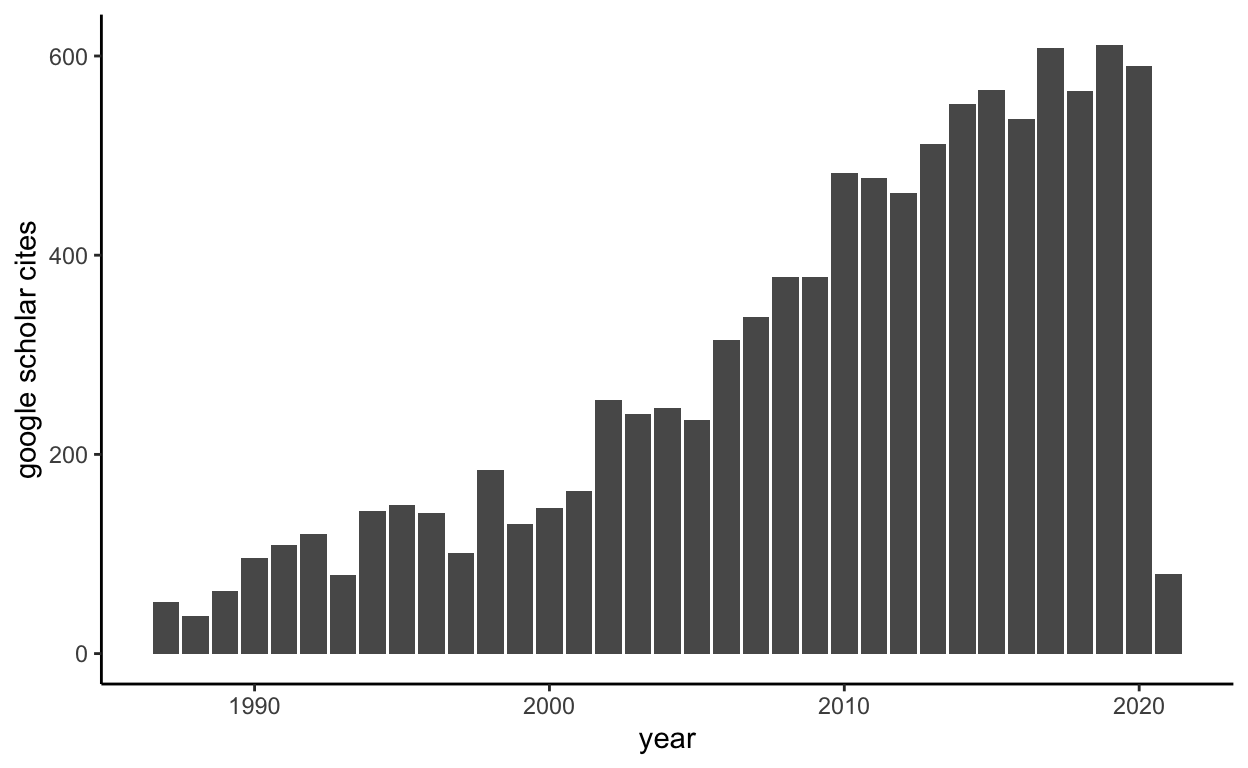
\includegraphics{cv.full_files/figure-latex/fig-margin1-1} \end{flushright}

\hypertarget{peer-reviewed-publications}{%
\subsection{5.2 Peer-reviewed
publications}\label{peer-reviewed-publications}}

\begin{enumerate}
\def\labelenumi{\arabic{enumi}.}
\item
  Rosenbaum, G., \textbf{Sandiford, M.}, Caulfield, J., Garrison, J.M.,
  in press, A trapdoor mechanism for slab tearing and melt generation in
  the northern Andes, Geology, \url{doi:10.1130/G45429.1}.
  \marginnote{citations  5}
\item
  Li, G., Kohn, B., \textbf{Sandiford, M.}, Ma, Z., Xu ,Z., 2018,
  Post-collisional exhumation of the Indus-Yarlung suture zone and
  Northern Tethyan Himalaya, SW Tibet, Gondwana Research 64, 1-10.
  \url{doi:10.1016/j.gr.2018.06.006}
\item
  Hoffman, N., Hardman-Mountford, N., Jenkins, C., Rayner,P.J., Gibson,
  G., \textbf{Sandiford, M.}, 2017, GipNet--Baseline Environmental Data
  Gathering and Measurement Technology Validation for Nearshore Marine
  Carbon Storage, Energy Procedia 114, 3729-3753.
  \url{doi:10.1016/j.egypro.2017.03.1503}.
\item
  Beardsmore, G., \textbf{Sandiford, M.}, Gordon, K., McLean, M., Egan,
  S. McLaren, S., 2017, Heat flow and inferred ground surface
  temperature history at Tynong North, southeastern Australia,
  Australian Journal of Earth Sciences, 64, 753-767,
  \url{doi:10.1080/08120099.2017.1362663}. \marginnote{citations  1}
\item
  Morell, K.D., \textbf{Sandiford, M.}, Kohn, B., Codilean, A., Folup,
  R., Ahmad, T., 2017, Current strain accumulation in the hinterland of
  the northwest Himalaya, Tectonophysics, 721, 70-89,
  \url{doi:10.1016/j.tecto.2017.09.007}. \marginnote{citations  11}
\item
  Li, G., Kohn, B., \textbf{Sandiford, M.}, Xu ,Z., 2017, India-Asia
  convergence: Insights from burial and exhumation of the Xigaze forearc
  basin, south Tibet, Journal of Geophysical Research, 122,
  \url{doi:10.1002/2017JB014080}. \marginnote{citations  15}
\item
  Boger, S.D., Spelbrink, L.G., Lee, R.I., \textbf{Sandiford, M.}, Maas,
  R., Woodhead, J.D., 2017, Isotopic (U-Pb, Nd) and geochemical
  constraints on the origins of the Aileu and Gondwana sequences of
  Timor, Journal of Asian Earth Sciences, 134, 330-351,
  \url{doi:10.1016/j.jseaes.2016.11.026}. \marginnote{citations  7}
\item
  Li, G., Kohn, B., \textbf{Sandiford, M.}, Xu ,Z., Seiler, C., Tian,
  Y., 2016, Synorogenic morphotectonic evolution of the Gangdese
  batholith, South Tibet: Insights from low-temperature
  Thermochronology, Geochemistry, Geophysics, Geosystems 17, 101-112.
  \url{doi:10.1002/2015GC006047}. \marginnote{citations  29}
\item
  Lawrie, K., Brodie, R.S. Christensen, N., Gibson, D., Halas, L.,
  Symington, N., Tan,K., \textbf{Sandiford, M.}, Ziramov, S., Urosevic,
  M., Grunewald, E., Hayes,P. 2016, Neotectonic Intra-Plate Fault Zone
  Mapping and Hydrogeology in Floodplain Sediments: An
  Inter-Disciplinary Approach, ASEG Extended Abstracts 2016, 1-9,
  \url{doi:10.1071/ASEG2016ab400}. \marginnote{citations  1}
\item
  Rajendran. C.P., Sanwal, J., Morell, K.D., \textbf{Sandiford, M.},
  Kotlia, B.S., Hellstrom, J., Rajendran, K., 2016, Stalagmite growth
  perturbations from the Kumaun Himalaya as potential earthquake
  recorders, Journal of Seismology, 20, 579-594.
  \marginnote{citations  16}
\item
  McConnell, D., Forcey, T., \textbf{Sandiford, M.}, 2015, Estimating
  the value of electricity storage in an energy-only wholesale market,
  Applied Energy, 159, 422-432 \url{doi:10.1016/j.apenergy.2015.09.006}.
  \marginnote{citations  76}
\item
  Coblentz, D., van Wijk, J., Richardson, R.M., \textbf{Sandiford, M.},
  2015, The Upper Mantle Geoid: Implications for Continental Structure
  and the Intraplate Stress Field. The Interdisciplinary Earth: A volume
  in honor of Don L. Anderson, Geological Society of America Special
  Paper 514, 197-214, ed.~G.R. Foulger, M. Lustrino and S. King.
  \url{doi:10.1130/2015.2514(13)} \marginnote{citations  9}
\item
  \textbf{Sandiford, M.}, Forcey, T., Pears, A., McConnell, D., 2015,
  Five years of declining annual consumption of grid-supplied
  electricity in eastern Australia: causes and consequences, The
  Electricity Journal, 28, 96-117, \url{doi:10.1016/j.tej.2015.07.007}
  \marginnote{citations  19}
\item
  Li, G., Kohn, B., \textbf{Sandiford, M.}, Xu, Z., We, L., 2015,
  Constraining the age of Liuqu Conglomerate, southern Tibet:
  Implications for evolution of the India-Asia collision zone. Earth and
  Planetary Science Letters, 426, 259-266,
  \url{doi:10.1016/j.epsl.2015.06.010} \marginnote{citations  33}
\item
  Li, G., Tian, Y., Kohn, B.P., \textbf{Sandiford, M.}, Xu, Z.,Ca, Z.,
  2015, Cenozoic low temperature cooling history of the Northern Tethyan
  Himalaya in Zedang, SE Tibet and its implications, Tectonophysics,
  \url{doi:10.1016/j.tecto.2014.12.014} \marginnote{citations  29}
\item
  Li., G., \textbf{Sandiford, M.}, Boger, S., Liu, X.., Wei, L., 2015,
  Provenance of the Upper-Cretaceous to Lower Tertiary sedimentary
  relicts in the Renbu mélange zone, within the Indus-Yarlung suture
  zone, Journal of Geology, 123, 39--54, \url{doi:10.1086/680207}
  \marginnote{citations  13}
\item
  Morell, K.D., \textbf{Sandiford, M.}, Rajendran, C.P., Rajendran, K.,
  Fink, D., Alimanovic, A., Sanwal, J., 2015, Geomorphology reveals
  active decollement geometry in the central Himalayan seismic gap,
  Lithosphere, 7, 247-256, \url{doi:10.1130/L407.1}
  \marginnote{citations  34}
\item
  Ely, K.S., \textbf{Sandiford, M.}, Phillips, D., Boger, S.D., 2014,
  Detrital zircon U-Pb and 40Ar/39Ar hornblende ages from the Aileu
  Complex, Timor-Leste: provenance and metamorphic cooling history,
  Journal of the Geological Society of London, doi: 10.1144/jgs2012-065
  \marginnote{citations  14}
\item
  Holford, S., Tuitt, A., Hillis, R., Green, P., Stoker, M., Duddy, I.,
  \textbf{Sandiford, M.}, Tassone, D., 2014, Cenozoic deformation in the
  Otway Basin, southern Australian margin: implications for the origin
  and nature of post-breakup compression at rifted margins, Basin
  Research, 26, 10--37, doi: 10.1111/bre.12035
  \marginnote{citations  46}
\item
  Li, G., \textbf{Sandiford, M.}, Liu, X., Xu, Z., We, L., Li. H., 2014,
  Provenance of the Late Triassic sediments in Central Lhasa terrane,
  Tibet, and its implication, Gondwana Research,
  \url{doi:10.1016/j.gr.2013.06.019} \marginnote{citations  53}
\item
  Rawling, T.J., \textbf{Sandiford, M.}, Beardsmore, G.R., Quenette, S.,
  Goyen, S.H., Harrison, B., 2014, Thermal insulation and geothermal
  targeting, with specific reference to coal-bearing basins, Australian
  Journal of Earth Sciences, 60, 817-830,
  \url{doi:10.1080/08120099.2013.864999} \marginnote{citations  8}
\item
  Rajendran, C.P., Rajendran, K., Sanwal, J., \textbf{Sandiford, M.},
  2013, Archeological and historical database on the medieval
  earthquakes of the central Himalaya: Ambiguities and Inferences,
  Seismological Research Letters, 84, 1098-1108, doi: 10.1785/0220130077
  \marginnote{citations  40}
\item
  Egholm, D., Knusden, M.F., \textbf{Sandiford, M.}, 2013, Lifespan of
  mountain ranges scaled by feedbacks between landsliding and erosion by
  rivers, Nature, 498, 475--478, \url{doi:10:1038/nature12218}
  \marginnote{citations  107}
\item
  Sanwal, J., Kotlia, B.S., Rajendran, C.P., Ahmad, S., Rajendran, K.,
  and \textbf{Sandiford, M.}, 2013, Climate variability in Central
  Indian Himalaya during the last \textasciitilde1,800 years: Evidence
  from high resolution speleothem record, Quaternary International, 304,
  183--192, \url{doi:/10.1016/j.quaint.2013.03.029}
  \marginnote{citations  72}
\item
  McConnell, D., Hearps, P., Eales, D., \textbf{Sandiford, M.}, Dunn,
  R., Wright, M., Bateman, L., 2013, Retrospective modeling of the
  merit-order effect on wholesale electricity prices from distributed
  photovoltaic generation in the Australian National Electricity Market,
  Energy Policy, 58,17-27, \url{doi:10.1016/j.enpol.2013.01.052}
  \marginnote{citations  104}
\item
  Shin, J., \textbf{Sandiford, M.}, 2012, Neogene uplift in the Korean
  peninsula linked to small-scale mantle convection at sinking slab
  edge. Journal of Korean Geographical Society, 47(3), 328-346
\item
  Turner, S., Caulfield, J., Turner, M., van Keken, P., Maury, R.,
  \textbf{Sandiford, M.}, Prouteau, G., 2012, Recent contribution of
  sediments and fluids to the mantle's volatile budget, Nature
  geoscience, 5, 50-54, \url{doi:10.1038/ngeo1325}
  \marginnote{citations  44}
\item
  Long, A., Budd, A., Gurgenci,H., Hand,M., Huddlestone-Holmes, C.,
  Leary ,P., Malin, P., Moghtaderi,B., Regenauer-Lieb,K.,
  \textbf{Sandiford, M.}, Webster, R., 2011, Australian geothermal
  research 2011, Proceedings, Thirty-Sixth Workshop on Geothermal
  Reservoir Engineering, Stanford University, Stanford, California,
  January 31 - February 2, 2011, SGP-TR-191
\item
  Clark, D., Cupper, M., \textbf{Sandiford, M.}, Kiernan, K., 2011,
  Style and timing of late Quaternary faulting on the lake Edgar Fault,
  southwest Tasmania, Australia: implications for hazard assessment in
  intracratonic areas, In: \textbackslash\$emard, F., Michetti, A.,
  Macalpin, J. (eds) Geological criteria for evaluating seismicity
  revisited: 40 years of paleoseismic investigations and the natural
  record of past earthquakes, Geological Society of AmericaSpecial
  Papers, 479, 109-131, \url{doi:10.1130/2011.2479(05)}
  \marginnote{citations  34}
\item
  Ely, K.S., \textbf{Sandiford, M.}, Hawke, M.L., Phillips, D., Quigley,
  M., dos Reis, J.E., Evolution of Ataúro Island: temporal constraints
  on subduction processes beneath the Wetar Zone, Banda Arc , Journal of
  Asian Earth sciences, \url{doi:10.1016/j.jseaes.2011.01.019}
  \marginnote{citations  20}
\item
  Holford, S.P., Hillis, R.R., Hand, M. and \textbf{Sandiford, M.},
  2011, Thermal weakening localizes intraplate deformation along the
  southern Australian continental margin, Earth and Planetary Science
  Letters, 305, 217-214, \url{doi:10.1016/j.epsl.2011.02.056}
  \marginnote{citations  49}
\item
  Fu,B., Walker, R., \textbf{Sandiford, M.}, 2011, The 2008 Wenchuan
  earthquake and active tectonics of Asia, Journal of Asian Earth
  Sciences, 40, 797-804 \marginnote{citations  17}
\item
  Jakica, S, Quigley, M., \textbf{Sandiford, M.}, Clark, D., Fifield,
  L.K., Alimanovic, A., 2011, Geomorphic and cosmogenic nuclide
  constraints on escarpment evolution in an intraplate setting, Darling
  Escarpment, Western Australia, Earth Surface Processes and Landforms,
  36, 449-459, \url{doi:10.1002/esp.2058} \marginnote{citations  27}
\item
  Turner, S., \textbf{Sandiford, M.}, Regan, M., Hawkesworth, C.,
  Hildreth, W., 2010, The origins of large volume, compositionally-zoned
  volcanic eruptions - new constraints from U-series isotopes and
  numerical thermal modeling for the 1912 Katmai-Novarupta eruption,
  Journal of Geophysical Research, 115, B12201,
  \url{doi:10.1029/2009JB007195} \marginnote{citations  14}
\item
  Quigley, M.C., Clark, D., \textbf{Sandiford, M.}, 2010, Tectonic
  geomorphology of Australia, In: Bishop, P., Pillans, B. (eds)
  Australian Landscapes. Geological Society, London, Special
  Publications, 346, 243-265 \marginnote{citations  109}
\item
  Quigley, M., Horton, T., Hellstrom, J., Cupper, M., \textbf{Sandiford,
  M.}, 2010, Holocene precipitation variability in arid Australia from
  speleothem and alluvial records, The Holocene,
  \url{doi:10.1177/0959683610369508} \marginnote{citations  63}
\item
  \textbf{Sandiford, M.}, 2010, Complex Subduction, Nature Geoscience,
  3, 518-520, \url{doi:10.1038/ngeo928} \marginnote{citations  6}
\item
  Brown, M., White, R.W., \textbf{Sandiford, M.}, 2010, On the
  importance of minding one's Ps and Ts: Metamorphic processes and
  quantitative petrology, Journal of Metamorphic Geology, 28, 561--567,
  \url{doi:10.1111/j.1525-1314.2010.00892.x} ",
\item
  \textbf{Sandiford, M.}, 2010, Why are the continents just so \ldots?,
  Journal of Metamorphic Geology, 28, 569--577
  \url{doi:10.1111/j.1525-1314.2010.00888.x} \marginnote{citations  11}
\item
  Farrington, R., Stegman, D., Moresi, L.N., \textbf{Sandiford, M.},
  May, D., 2010, Interactions of 3D mantle flow and continental
  lithosphere near passive margins, Tectonophysics, 483, 20-28
  \url{doi:10.1016/j.tecto.2009.10.008} \marginnote{citations  40}
\item
  Ely, K., \textbf{Sandiford, M.}, 2010, Seismic response to slab
  rupture and variation in lithospheric structure beneath the Savu Sea,
  Indonesia, Tectonophysics, 483, 112-124,
  \url{doi:10.1016/j.tecto.2009.08.027} \marginnote{citations  25}
\item
  Woodhead, J., Hergt, J., \textbf{Sandiford, M.}, Johnson, W., 2010,
  The big crunch: physical and chemical expressions of arc/continent
  collision in the western Bismarck arc, Journal of Volcanology and
  Geothermal Research, 190, 11-24
  \url{doi:10.1016/j.jvolgeores.2009.03.003} \marginnote{citations  36}
\item
  Quigley M. C., \textbf{Sandiford, M.}, Clark, D., 2009, Neotectonics
  and landscape evolution of southeastern Australia: establishing a
  geologic context for contemporary seismicity, In: Clark, D., (ed),
  Potential geologic sources of seismic hazard in the Sydney Basin.
  Geoscience Australia Record 2009/11, 1-6
\item
  \textbf{Sandiford, M.}, Quigley, M., de Broekert, P., Jakica, S.,
  2009, Tectonic framework for the Cenozoic cratonic basins of
  Australia, Australian Journal of Earth Sciences, 56, S5-S18,
  \url{doi:10.1080/08120090902870764} \marginnote{citations  63}
\item
  Turner,S., Haines, P., Foster, D, Powell R., \textbf{Sandiford, M.},
  Offler, R.,2009, Did the Delamerian Orogeny start in the
  Neoproterozoic? Journal of Geology, 117, 575-583
\item
  Braun, J., Burbidge, D.R., Gesto, F.N., \textbf{Sandiford, M.},
  Gleadow, A.J.W., Kohn, B.P., Cummins, P.R., 2009, Constraints on the
  current rate of deformation and surface uplift of the Australian
  continent from a new seismic database and low-T thermochronological
  data. Australian Journal of Earth Sciences, 56, 99-110
  \url{doi:10.1080/08120090802546977} \marginnote{citations  58}
\item
  McLaren, S., \textbf{Sandiford, M.}, Dunlap, W.J., Scrimgeour, I.,
  Close, D. and Edgoose, C., 2009, Distribution of Palaeozoic reworking
  in the Western Arunta province and northwestern Amadeus Basin from
  40Ar/39Ar thermochronology: implications for the evolution of
  intracratonic basins, Basin Research, 21, 315-334
  \url{doi:10.1111/j.1365-2117.2008.00385.x} \marginnote{citations  21}
\item
  \textbf{Sandiford, M.}, Quigley,M.C., 2009, TOPO-OZ: insights into the
  various modes of intraplate deformation in the Australian continent,
  Tectonophysics, 474, 405-416 \url{doi:10.1016/j.tecto.2009.01.028}
  \marginnote{citations  62}
\item
  Somerville, P., Quijada, P., Hong Kie Thio, \textbf{Sandiford, M.},
  Quigley, M., 2008, Contribution of identified active faults to near
  fault seismic hazard in the Flinders Ranges, Australian Earthquake
  Engineering Society Conference Proceedings, Paper 45, 1-9.
\item
  Egholm, D.L., Clausen, O.R., \textbf{Sandiford, M.}, Kristensen, M.B.,
  Korstgard, J.A., 2008, The mechanics of clay smearing along faults,
  Geology, 36, 787--790 \url{doi:0.1130/G24975A.1}
  \marginnote{citations  74}
\item
  Hillis, R.R., \textbf{Sandiford, M.}, Reynolds, S.D. and Quigley,
  M.C., 2008, Present-day stresses, seismicity and Neogene-to-Recent
  tectonics of Australia's `passive' margins: intraplate deformation
  controlled by plate boundary forces. In: Johnson, H., Dore, A. G.,
  Gatliff, R. W., Holdsworth, R., Lundin, E. and Ritchie, J. D. (eds)
  The Nature and Origin of Compression in Passive Margins. Geological
  Society, London, Special Publications, 306, 71--89
  \url{doi:10.1144/SP306.3} \marginnote{citations  157}
\item
  \textbf{Sandiford, M.}, Egholm, D.L., 2008, Enhanced intraplate
  seismicity along continental margins: some causes and consequences,
  Tectonophysics, 457, 197--208, \url{doi:10.1016/j.tecto.2008.06.004}
  \marginnote{citations  49}
\item
  Quigley, M.C., Yu Liangjun, Gregory, C., Corvino, A.,
  \textbf{Sandiford, M.}, Wilson, C.J.L., Liu Xiaohan, 2008, U-Pb SHRIMP
  zircon geochronology and T-t-d history of the Kampa Dome, southern
  Tibet, Tectonophysics, 446, 97-113
  \url{doi:10.1016/j.tecto.2007.11.004} \marginnote{citations  88}
\item
  Dosseto, A., Turner, S.P., \textbf{Sandiford, M.}, Davidson, J., 2008,
  Uranium-series isotope and thermal constraints on the rate and depth
  of silicic magma genesis, In: Dynamics of Crustal Magma Transfer,
  Storage and Differentiation, Annen C. and Zellmer, G.F. (eds).
  Geological Society of London Special Publication, 304, 169-181
  \marginnote{citations  9}
\item
  Hou, B., Frakes, L.A., \textbf{Sandiford, M.}, Worrall, L., Keeling,
  J., Alley, N.F., 2008, Cenozoic Eucla Basin and associated
  palaeovalleys, southern Australia - climatic and tectonic influences
  on landscape evolution, sedimentation and heavy mineral accumulation,
  Sedimentary Geology, 203, 112-130 doi: 10.1016/j.sedgeo.2007.11.005
  \marginnote{citations  69}
\item
  \textbf{Sandiford, M.}, 2008, Seismic moment release during slab
  rupture beneath the Banda Sea, Geophysical Journal International, 174,
  659--671 doi: 10.1111/j.1365-246X.2008.03838.x
  \marginnote{citations  34}
\item
  Bowler, J.M., \textbf{Sandiford, M.}, 2007, Dynamic Antarctic Ice:
  agent for Mid-Pleistocene Transition, PAGESnews, 15, 16-18
  \marginnote{citations  3}
\item
  Quigley, M., \textbf{Sandiford, M.}, Cupper, M., 2007, Distinguishing
  tectonic from climatic controls on range-front sedimentation, Flinders
  Ranges, South Australia. Basin Research, 19, 491--505 doi:
  10.1111/j.1365-2117.2007.00336.x \marginnote{citations  77}
\item
  Demidjuk, Z., Turner, S., \textbf{Sandiford, M.}, George, R., Foden,
  J., Etheridge, M., 2007, U-series isotope and geodynamic constraints
  on mantle melting processes beneath the Newer Volcanic Province in
  South Australia, Earth and Planetary Science Letters, 261, 517--533
  doi: 10.1016/j.epsl.2007.07.006 \marginnote{citations  112}
\item
  \textbf{Sandiford, M.}, 2007, The tilting continent: a new constraint
  on the dynamic topographic field from Australia, Earth and Planetary
  Science Letters, 261, 152-163 doi: 10.1016/j.epsl.2007.06.023
  \marginnote{citations  118}
\item
  Quigley, M., \textbf{Sandiford, M.}, Alimanovic, A., Fifield, L.K.,
  2007, Landscape responses to intraplate tectonism in the Flinders
  Ranges, South Australia: quantitative constraints from 10Be
  abundances, Earth and Planetary Science Letters, 261,120-133
  \url{doi:10.1016/j.epsl.2007.06.020} \marginnote{citations  50}
\item
  Egholm, D.L., \textbf{Sandiford, M.}, Clausen, O.L., Nielsen, S.B.,
  2007, A new strategy for discrete element numerical models Part II:
  Sandbox applications, Journal of Geophysical Research, 112, B05204
  \url{doi:10.1029/2006JB004558} \marginnote{citations  69}
\item
  Quigley, M., \textbf{Sandiford, M.}, Fifield, K., Alimanovic A., 2007,
  Bedrock erosion and relief production in the northern Flinders Ranges,
  Australia. Earth Surface Processes and Landforms, 32, 929-944 doi:
  10.1002/esp.1459 \marginnote{citations  69}
\item
  McLaren, S., \textbf{Sandiford, M.}, Powell, R., Neumann, N.,
  Woodhead, J., 2006, Palaeozoic intraplate crustal anatexis in the
  Mount Painter province, South Australia: timing, thermal budgets and
  the role of crustal heat production, Journal of Petrology, 47,
  2281-2302 \url{doi:10.1093/petrology/egl044}
  \marginnote{citations  65}
\item
  Quigley, M., Yu Liangjun, Liu Xiaohan, Wilson, C.J.L,
  \textbf{Sandiford, M.}, Phillips, D., 2006, 40Ar/39Ar thermochronology
  of the Kampa Dome, southern Tibet: implications for the thermal
  evolution of North Himalayan middle crust, Tectonophysics, 421,
  269-297 \marginnote{citations  61}
\item
  Nelson, E., Hillis, R., \textbf{Sandiford, M.}, Reynolds, S., Lyon,
  P., Meyer, J., Mildren, S., Rogers, C., 2006, Present-day
  state-of-stress of southeast Australia, APPEA Journal 2006, 283-305
\item
  Grew, E.S., Yates, M.G.,Shearer, C.K., Hagerty, J.J., Sheraton, J.W.,
  \textbf{Sandiford, M.}, 2006, Beryllium and other trace elements in
  paragneisses and anatectic veins of the ultrahigh-temperature Napier
  Complex, Enderby Land, East Antarctica: the role of sapphirine,
  Journal of Petrology, 47, 859-882 \url{doi:10:1093/petrology/egi098}
  \marginnote{citations  29}
\item
  \textbf{Sandiford, M.}, McLaren, S., 2006, Thermo-mechanical controls
  on heat production distributions and the long-term evolution of the
  continents, ``Evolution and differentiation of the continental crust''
  (eds, Brown, M. and Rushmer, T.), Cambridge University Press, 67-91
  \marginnote{citations  30}
\item
  Quigley, M., Cupper, M., \textbf{Sandiford, M.}, 2006, Quaternary
  faults of south-central Australia: palaeoseismicity, slip rates and
  origin, Australian Journal of Earth Sciences, 53, 285-301
  \marginnote{citations  119}
\item
  Bodorkos, S., \textbf{Sandiford, M.}, 2006, Thermal and mechanical
  controls on the evolution of Archean crustal deformation: examples
  from Western Australia, AGU Volume Archean Geodynamic and
  Environments, (eds, Keith Benn, Jean-Cl\textbackslash\$e Mareschal,
  Kent Condie). Geophysical Monograph Series 164, American Geophysical
  Union), 370 \marginnote{citations  32}
\item
  \textbf{Sandiford, M.}, Hansen D.L., McLaren, S.N., 2006, Lower
  crustal rheological expression in inverted basins, in Analogue and
  Numerical Modelling of Crustal Scale Processes (eds Buiter, S. and
  Schreurs, G.). Geological Society Special Publication, 253, 271-283
\item
  Celerier, J., \textbf{Sandiford, M.}, Hansen, D.L., Quigley, M., 2005,
  Modes of active intraplate deformation, Flinders Ranges, Australia,
  Tectonics, 24 \url{doi:10.029/2004andC001679}
  \marginnote{citations  113}
\item
  McLaren, S., \textbf{Sandiford, M.}, Powell, R., 2005, Contrasting
  styles of Proterozoic crustal evolution: a hot-plate tectonic model
  for Australian terranes, Geology, 33,673-676
  \marginnote{citations  76}
\item
  Wallace, M., Dickinson, J.A., Moore, D., \textbf{Sandiford, M.}, 2005,
  Late Neogene strandlines of Southern Victoria: A unique record of
  eustasy and tectonics in southeast Australia, Australian Journal of
  Earth Sciences, 52, 277-295. \marginnote{citations  71}
\item
  de Broekert, P., \textbf{Sandiford, M.}, 2005, Buried inset-valleys in
  the eastern Yilgarn Craton, Western Australia: Geomorphology, age and
  allogenic control, Journal of Geology, 113, 471-493
\item
  \textbf{Sandiford, M.}, Coblentz, D., Schellart, W.P., 2005,
  Evaluating slab-plate coupling in the Indo-Australian plate, Geology,
  33, 113-116 \marginnote{citations  36}
\item
  \textbf{Sandiford, M.}, Wallace, M., Coblentz, D, 2004, Origin of the
  in situ stress field in south-eastern Australia, Basin Research, 16,
  325-338
\item
  \textbf{Sandiford, M.}, Van Kranendonk, M., Bodorkos, S., 2004,
  Conductive incubation and the origin of granite-greenstone dome and
  keel structure: the Eastern Pilbara Craton, Australia, Tectonics, 23,
  TC1009, doi: 10.1029/2002TC001452 \marginnote{citations  75}
\item
  Bodorkos, S., \textbf{Sandiford, M.}, Minty, B.R.S., Blewett, R.S.,
  2004, A high-resolution, calibrated airborne radiometric dataset
  applied to the estimation of crustal heat production in the Archaean
  northern Pilbara Craton, Western Australia, Precambrian Research, 128,
  57-82
\item
  \textbf{Sandiford, M.}, Leonard, M., Coblentz, D, 2003, Geological
  constraints on active seismicity in southeast Australia, In
  ``Earthquake Risk Mitigation'', (eds, Wilson, J.L, Lam, N.K., Gibson.
  G.), Australian Earthquake Engineering Society, 1-10
\item
  \textbf{Sandiford, M.}, Frederiksen, S., Braun, J., 2003, The
  long-term thermal consequences of rifting: implications for basin
  reactivation, Basin Research,15, 23-43 \marginnote{citations  20}
\item
  \textbf{Sandiford, M.}, 2003, Geomorphic constraints on the late
  Neogene tectonics of the Otway Range, Victoria, Australian Journal of
  Earth Sciences, 50, 69-80 \marginnote{citations  83}
\item
  McLaren, S., \textbf{Sandiford, M.}, Hand, M., Neumann, N., Wyborn,
  L., Bastrakova, I., 2003, The hot southern continent, Heat flow and
  heat production in Australian Proterozoic terranes, eds Hillis, R.R.
  Muller, D., Evolution and dynamics of the Australian Plate, Geological
  Society of Australia, Special Publication, 22, 151-161
  \marginnote{citations  117}
\item
  \textbf{Sandiford, M.}, 2003, Neotectonics of southeastern Australia:
  linking the Quaternary faulting record with seismicity and in situ
  stress, eds Hillis, R.R. Muller, D., Evolution and dynamics of the
  Australian Plate, Geological Society of Australia, Special
  Publication, 22, 101-113 \marginnote{citations  204}
\item
  \textbf{Sandiford, M.}, 2002, Late Neogene faulting record in
  southeastern Australia, In Victoria Undercover, (eds.~Phillips, G.N.,
  and Ely, K.S.,), 131-135
\item
  \textbf{Sandiford, M.}, McLaren, S., 2002, Tectonic feedback and the
  ordering of heat producing elements within the continental
  lithosphere, Earth and Planetary Science Letters, 2002, 204, 133-150
  \marginnote{citations  164}
\item
  \textbf{Sandiford, M.},2002, Low thermal Peclet number intraplate
  orogeny in central Australia, Earth and Planetary Science Letters,201,
  309-320. \marginnote{citations  28}
\item
  Foden, J.D., Elburg, M.A., Turner, S.P., \textbf{Sandiford, M.},
  O'Callghan, J., Mitchell, S., 2002, Granite production in the
  Delamerian Orogen, South Australia, Journal of the Geological society
  of London, 159, 557-575 \marginnote{citations  101}
\item
  McLaren, S., Dunlap, J., \textbf{Sandiford, M.} McDougall, I., 2002,
  The thermochronology of high heat-producing crust at Mount Painter,
  South Australia: implications for tectonic reactivation of continental
  interiors, Tectonics \url{doi:10.1029/2000TC001275}
  \marginnote{citations  76}
\item
  Alías, G., \textbf{Sandiford, M.}, Hand, M., Worley, B., 2002, The P-T
  record of synchronous magmatism, metamorphism and deformation at
  Petrel Cove, southern Adelaide Fold Belt, Journal of Metamorphic
  Geology, 20, 351-36 \marginnote{citations  24}
\item
  Bodorkos, S., \textbf{Sandiford, M.}, Oliver, N.H.S., Cawood, P.A.
  2002, High-T, low-P metamorphism as the middle crustal response to a
  mantle-related transient thermal pulse: a numerical model and its
  application to the Palaeoproterozoic Halls Creek Orogen, northern
  Australia, Journal of Metamorphic Geology, 20, 217-237
  \marginnote{citations  47}
\item
  \textbf{Sandiford, M.}, McLaren, S., Neumann, N, 2002, Long-term
  thermal consequences of the redistribution of heat-producing elements
  associated with large-scale granitic complexes, Journal of Metamorphic
  Geology, 20, 87-98 \marginnote{citations  83}
\item
  Haines, P, Hand, M., \textbf{Sandiford, M.}, 2001, Palaeozoic
  syn-orogenic sedimentation in central and northern Australia: a review
  of distribution and timing with implications for the evolution of
  intracontinental orogens, Australian Journal of Earth Sciences, 48,
  911-928 \marginnote{citations  178}
\item
  \textbf{Sandiford, M.}, Hand, M.,McLaren, S., 2001, Tectonic feedback,
  intraplate orogeny and the geochemical structure of the crust: a
  central Australian perspective, In Continental Reactivation and
  Reworking, (eds, Miller, J., Holdsworth, R., Buick, I., Hand, M.),
  Geological Society Special Publication No.~184, 195-218
  \marginnote{citations  82}
\item
  McLaren, S., \textbf{Sandiford, M.}, 2001, Long-term thermal
  consequences of tetconic activity at Mount Isa, Australia:
  Implications for polyphase tectonism in the Proterozoic.In Continental
  Reactivation and Reworking, (eds, Miller, J., Holdsworth, R., Buick,
  I., Hand, M.), Geological Society Special Publication No.~184, 219-236
  \marginnote{citations  21}
\item
  Neumann, N, \textbf{Sandiford, M.}, Foden, J., 2000, Regional
  geochemistry and continental heat flow: Implications for the origin of
  the South Australian heat flow anomaly. Earth and Planetary Science
  Letters, 183, 107-120 \marginnote{citations  175}
\item
  Fraser, G., Worley, B., \textbf{Sandiford, M.}, 2000, High‐precision
  geothermobarometry across the High Himalayan metamorphic sequence,
  Langtang Valley, Nepal. Journal of metamorphic Geology,18, 665 - 682
  \marginnote{citations  90}
\item
  McLaren, S., \textbf{Sandiford, M.}, Hand, M., 2000, High radiogenic
  heat producing granites and metamorphism - an example from the western
  Mount Isa Inlier, Australia, reply to comment, Geology, 28, 672
  \marginnote{citations  123}
\item
  Paul, E., \textbf{Sandiford, M.}, Flottman, T., 2000, The structural
  geometry of a thick-skinned fold-thrust belt termination : the Olary
  Block in the Adelaide Fold Belt, South Australia. Australian Journal
  of Earth Sciences, 47, 281-290 \marginnote{citations  24}
\item
  Arnold, J., Powell, R., \textbf{Sandiford, M.}, 2000, Amphibolites
  with staurolite and other aluminous minerals: calculated mineral
  equilibria in NCFMASH, Journal of metamorphic Geology, 18, 23-40
  \marginnote{citations  25}
\item
  McLaren, S., \textbf{Sandiford, M.}, Hand, M., 1999, High radiogenic
  heat producing granites and metamorphism - an example from the western
  Mount Isa Inlier, Australia, Geology, 27, 679-682
  \marginnote{citations  123}
\item
  Hand, M., \textbf{Sandiford, M.}, Wyborn, L., 1999, Some thermal
  consequences of high heat production in the Australian Proterozoic.
  AGSO research Newsletter, 30, 20-23 \marginnote{citations  15}
\item
  McLaren, S., Neumman, N., \textbf{Sandiford, M.}, Wyborn, L., 1999,
  Post-intrusion heating associated with high-heat-producing Proterozoic
  granites - Implications for mineralisation? AGSO research Newsletter,
  30, 23-26 \marginnote{citations  10}
\item
  Tokarev, V., \textbf{Sandiford, M.}, Gostin, V., 1999, Landscape
  evolution in the Mount Lofty Ranges: implications for regolith
  development. In Regolith'98 : new approaches to an old continent,
  (eds) Taylor, G., Pain C., 131-139. \marginnote{citations  32}
\item
  Hand, M., \textbf{Sandiford, M.}, 1999, Intraplate deformation in
  central Australia, the link between subsidence and fault ractivation,
  Tectonophysics, 305, 121-140 \marginnote{citations  175}
\item
  \textbf{Sandiford, M.}, 1999, Mechanics of basin inversion,
  Tectonophysics, 305, 109-120 \marginnote{citations  82}
\item
  Paul, E., Flottmann, T., \textbf{Sandiford, M.}, 1999, Structural
  geometry and controls on basement-involved deformation in the northern
  Flinders Ranges, Adelaide Fold Belt, South Australia, Australian
  Journal of Earth Sciences, 46, 343-354 \marginnote{citations  71}
\item
  Foden, J., \textbf{Sandiford, M.}, Dougherty-Page, J., Willliams, I.,
  1999, Geochemistry and geochronology of the Rathjen Gneiss:
  implications for the early tectonic evolution of the Delamerian
  Orogen. Australian Journal of Earth Science, 46, 377-389
  \marginnote{citations  94}
\item
  \textbf{Sandiford, M.}, Paul, E., Flottmann, T., 1998, Sedimentary
  thickness variations and deformation intensity during basin inversion
  in the Flinders Ranges, South Australia, Journal of Structural
  Geology, 20, 1721-1731 \marginnote{citations  28}
\item
  \textbf{Sandiford, M.}, Hand, M., McLaren, S., 1998, High geothermal
  gradient metamorphism during thermal subsidence, Earth and Planetary
  Science Letters, 163, 149-165 \marginnote{citations  122}
\item
  \textbf{Sandiford, M.}, Hand, M., 1998, Controls on the locus of
  Phanerozoic intraplate deformation in central Australia, Earth and
  Planetary Science Letters, 162, 97-110 \marginnote{citations  166}
\item
  Coblentz, D., Zhou, S., Hillis, R., Richardson, R., \textbf{Sandiford,
  M.}, 1988, Topography, plate-boundary forces and the Indo-Australian
  intraplate stress field, Journal of Geophysical Research, 103, 919-931
  \marginnote{citations  196}
\item
  \textbf{Sandiford, M.}, Hand, M., 1998, Australian Proterozoic
  high-temperature metamorphism in the conductive limit, In What
  Controls Metamorphism, (ed) Treloar, P., and O'Brien, P, Geological
  Society of London Special Publication, 138, 103-11
  \marginnote{citations  54}
\item
  Hillis, R., \textbf{Sandiford, M.}, Coblentz, D., Zhou, S., 1997,
  Modelling the Contemporary stress field and its implications for
  Hydrocarbon exploration, Exploration Geophysics, 28, 88-93
  \marginnote{citations  12}
\item
  Turner, S., Kelly, S.P, Vandenberg, A.H., Foden, J.,
  \textbf{Sandiford, M.}, Flotmmann, T., 1996, Source of Delamerian fold
  belt flysch linkes to convective removal of the lithospheric mantle
  and rapid exhumation of the Delamerian-Ross fold belt, Geology, 24,
  941-944 \marginnote{citations  102}
\item
  Zhou, S., Hillis, R , \textbf{Sandiford, M.}, 1996, A supplement to `A
  study of inclined wellbores with regard to both mechanical stability
  and fracture intersection and its application to the Australian North
  West Shelf', Journal of Applied Geophysics, 36,
  145-147.\marginnote{citations  2}
\item
  Zhou, S., Hillis, R , \textbf{Sandiford, M.}, On the mechanical
  stability of inclined boreholes, SPE drilling, 11, 67-73.
  \marginnote{citations  54}
\item
  Turner, S., \textbf{Sandiford, M.}, Flottman, T., Foden, J., 1995,
  Rb/Sr dating of differentiated cleavage from the Adelaidean
  metasediments at Hallet Cove, southern Adelaide Fold Belt: Reply to
  disucssion by W.V. Preiss, Journal of Structural Geology, 17,
  1801-1803.\\
\item
  Arnold, J., \textbf{Sandiford, M.}, Wetherley, S., 1995, Metamorphic
  events in the Eastern Arunta Inlier, Part 1. Metamorphic petrology,
  Precambrian Research,71, 183-205. \marginnote{citations  21}
\item
  Coblentz, D., \textbf{Sandiford, M.}, Richardson, R, Zhou, S., Hillis,
  R., 1995, The origins of the Australian stress field, Earth and
  Planetary Science Letters, 133, 299-309. \marginnote{citations  173}
\item
  \textbf{Sandiford, M.}, Coblentz, D., Richardson, R.M., 1995, Ridge
  torques and continental collision in the Indian-Australian plate,
  Geology, 23, 653-656. \marginnote{citations  46}
\item
  Stuwe, K., \textbf{Sandiford, M.}, 1995, Description of Metamorphic
  Pressure- Temperature-Time paths in the Low-P High-T Environment,
  Physics of the Earth and Planetary Interiors, 88, 211-221.\\
\item
  Stuwe, K., \textbf{Sandiford, M.}, 1995, Mantle lithospheric
  deformation and crustal metamorphism, with some speculations on the
  thermal and mechanical significance of the Tauern event, Eastern Alps,
  Tectonophysics, 214, 115-132. \marginnote{citations  17}
\item
  \textbf{Sandiford, M.}, Fraser, G., Arnold, J., Foden, J., Farrow, T.,
  1995, Some causes and consequences of high‐temperature, low‐pressure
  metamorphism in the eastern Mt Lofty Ranges, South Australia,
  Australian Journal of Earth Sciences, 42,
  233-240.\marginnote{citations  36}
\item
  Mildren, S., \textbf{Sandiford, M.}, 1995, A heat refraction mechanism
  for Low-P metamorphism in the northern Flinders Ranges, South
  Australia, Australian Journal of Earth Sciences, 42, 241-247.
  \marginnote{citations  31}
\item
  Cartwright, I., Vry, J., \textbf{Sandiford, M.}, 1995, Changes in
  stable isotope ratios of metapelites and marbles during regional
  metamorphism, Mount Lofty Ranges, South Australia: Implications for
  crustal scale fluid flow, Contributions to Mineralogy and Petrology,
  120, 292-310. \marginnote{citations  43}
\item
  Zhou, S., Hillis, R., \textbf{Sandiford, M.}, 1994, A study of
  inclined wellbores with regard to both mechanical stability and
  fracture intersection and its application to the Australian North West
  Shelf, Journal of Applied Geophysics, 32,
  293-304.\marginnote{citations  27}
\item
  Coblentz, D., \textbf{Sandiford, M.}, 1994, Tectonic stresses in the
  African plate: Constraints on the ambient stress state, Geology, 22,
  831-834. \marginnote{citations  108}
\item
  Coblentz, D., Richardson, R.M., \textbf{Sandiford, M.}, 1994, On the
  gravitational potential of the Earth's lithosphere, Tectonics, 13,
  929-945. \marginnote{citations  112}
\item
  Ehlers, K., Stuwe, K., Powell, R., \textbf{Sandiford, M.}, Frank, W.,
  1994, Thermometrically inferred cooling rates from the Plattengneis,
  Koralm Region - Eastern Alps, Earth and Planetary Science Letters,
  125, 307-321.\marginnote{citations  24}
\item
  \textbf{Sandiford, M.}, Coblentz, D., 1994, Plate-scale potential
  energy distributions and the fragmentation of ageing plates, Earth and
  Planetary Science Letters, 126, 143-159. \marginnote{citations  31}
\item
  Stuwe, K., \textbf{Sandiford, M.}, 1994, A possible contribution of
  deviatoric stresses to metamorphic PT paths; an example appropriate to
  low-P, high-T metamorphism, Journal of Metamorphic Geology, 12,
  445-454. \marginnote{citations  50}
\item
  Turner, S., \textbf{Sandiford, M.}, Flottman, T., Foden, J., 1994,
  Rb-Sr dating of differentiated cleavage: an example from the
  Adelaidean metasediments at Hallet Cove, with implications for the
  tectonic evolution of the southern Adelaide Fold Belt, Journal of
  Structural Geology, 16, 1233-1242. \marginnote{citations  25}
\item
  Stuwe, K., \textbf{Sandiford, M.}, 1994, Some remarks on the
  geomorphological evolution of the eastern Alps, constraints on
  Cretaceous nappe tectonics, Mitteilungen der Osterreichischen
  geologischen Gesellschaft, 86, 165-176. \marginnote{citations  7}
\item
  Stuwe, K., \textbf{Sandiford, M.}, 1993, A preliminary model for the
  500 Ma event in the East Antarctic Shield, In: Gondwana Eight
  (eds.~Findlay, Unrug and Veevers), Balkema, 125,
  \marginnote{citations  34}
\item
  Turner, S., Foden, J., \textbf{Sandiford, M.}, Bruce, D., 1993, Sm-Nd
  isotopic evidence for the provenance of sediments from the Adelaide
  Fold Belt and southeastern Australia with implications for crustal
  growth models, Geochemica Cosmochemica Acta, 57, 1837-1856.
  \marginnote{citations  121}
\item
  Stuwe, K., \textbf{Sandiford, M.}, Powell, R., 1993, Episodic
  metamorphism and deformation events in Low-P, High-T terrains,
  Geology, 21, 829-832. \marginnote{citations  56}
\item
  Scrimgeour, I., \textbf{Sandiford, M.}, 1993, Early Proterozoic
  metamorphism at the Granites, northern Territory, implications for
  fluid production in high T - low P terrains, Economic Geology, 88,
  1099-1113. \marginnote{citations  21}
\item
  Dymoke, P., \textbf{Sandiford, M.}, 1992, Phase relations in Buchan
  facies series pelitic assemblages: calculations with application to
  andalusite-staurolite assemblages in the Mount Lofty Ranges, South
  Australia, Contributions to Mineralogy and Petrology, 110, 121-132.
  \marginnote{citations  65}
\item
  Jenkins, R.F.J., \textbf{Sandiford, M.}, 1992, Observations on the
  tectonic evolution of the southern Adelaide fold Belt, Tectonophysics,
  214, 27-36. \marginnote{citations  71}
\item
  \textbf{Sandiford, M.}, Foden, J., Zhou, S., Turner, S., 1992, Granite
  genesis and the mechanics of convergent orogenic belts with
  application to the southern Adelaide Fold Belt. Proceedings of the
  Royal Society of Edinburgh (Hutton Symposium Volume) 83, 83-93.
  \marginnote{citations  64}
\item
  Zhou, S., \textbf{Sandiford, M.}, 1992, On the stability of
  isostatically compensated mountain belts. Journal of Geophysical
  Research, 97, 14207-14221. \marginnote{citations  65}
\item
  \textbf{Sandiford, M.}, Foden, J., Zhou, S., Turner, S., 1992, Granite
  genesis and the mechanics on convergent orogenic belts with
  application to the southern Adelaide Fold Belt. Geological Society of
  America, Special Paper, 273, 83-93.\marginnote{citations  64}
\item
  Turner, S., \textbf{Sandiford, M.}, Foden, J., 1992, Some geodynamic
  and compositional constraints on ``post-orogenic'' magmatism, Geology,
  20, 931-934. \marginnote{citations  286}
\item
  Ding, P., James, P., \textbf{Sandiford, M.}, 1992, Late Proterozoic
  deformation in the Amadeus Basin, central Australia. Australian
  Journal of Earth Sciences, 39, 495-500. \marginnote{citations  13}
\item
  \textbf{Sandiford, M.}, Santosh, M., 1991, A granulite facies
  kalsilite-leucite-hibonite association from Punalur, southern India.
  Mineralogy and Petrology, 43, 225-236.\marginnote{citations  28}
\item
  \textbf{Sandiford, M.}, Dymoke, P., 1991, Some remarks on the
  stability of blueschists and related high P - low T assemblages in
  continental orogens, Earth and Planetary Science Letters, 102, 14-23.
  \marginnote{citations  19}
\item
  \textbf{Sandiford, M.}, Powell, R., 1991, Some remarks on high
  temperature-low pressure metamorphism in convergent orogens, Journal
  of Metamorphic geology, 9, 333-340. \marginnote{citations  190}
\item
  Santosh, M., \textbf{Sandiford, M.}, Reed, S.J.B., 1991, Zoned
  hibonites from Punalur, South India, Mineralogical Magazine, 55,
  159-162. \marginnote{citations  10}
\item
  \textbf{Sandiford, M.}, Martin, N., Zhou, S., Fraser, G., 1991,
  Mechanical consequences of granite emplacement during high-T, low-P
  metamorphism and the origin of ``anticlockwise'' PT paths, Earth and
  Planetary Science Letters, 107, 164-172. \marginnote{citations  79}
\item
  \textbf{Sandiford, M.}, Oliver, R.L., Mills, K.J., Allen, R.V., 1990,
  A cordierite-staurolite- muscovite association east of Springton,
  Mount Lofty Ranges; implications for the metamorphic evolution of the
  Kanmantoo Group. In ``Proterozoic and early Palaeozoic geology of the
  Adelaide Geosyncline'', Geological Society of Australia, Special
  publication (Daily Volume), 16, 483-495.\marginnote{citations  23}
\item
  \textbf{Sandiford, M.}, Powell, R., 1990, Some thermal and isostatic
  consequences of the vertical strain geometry in convergent orogens,
  Earth and Planetary Science Letters, 98, 154 - 165.
  \marginnote{citations  105}
\item
  Arnold, J., \textbf{Sandiford, M.}, 1990, Petrogenesis of
  cordierite-orthoamphibole assemblages in the Springton region, South
  Australia, Contributions to Mineralogy and Petrology, 106, 100-109.
  \marginnote{citations  36}
\item
  \textbf{Sandiford, M.}, 1989, Horizontal structures in granulite
  terrains : a record of mountain building or mountain collapse?
  Geology, 17, 449 - 452. \marginnote{citations  144}
\item
  \textbf{Sandiford, M.}, 1989, Secular trends in the thermal evolution
  of metamorphic belts, Earth and Planetary Science Letters, 95, 85-96.
  \marginnote{citations  41}
\item
  Powell, R., \textbf{Sandiford, M.}, 1988, Sapphirine and spinel phase
  relationships in the system FeO-MgO-SiO2-TiO2-Al2O3-O2 in the presence
  of quartz and hypersthene. Contributions to Mineralogy and Petrology,
  98, 64-71.\marginnote{citations  63}
\item
  Waldron, W., \textbf{Sandiford, M.}, 1988, Deformation volume and
  cleavage development in metasediments from the Ballarat Slate Belt,
  Journal of Structural Geology, 10, 53-62.\marginnote{citations  48}
\item
  \textbf{Sandiford, M.}, Powell, R., Martin, S.F., Perera, L.R.K.,
  1988. Thermal and baric evolution of garnet granulites, Sri Lanka.
  Journal of Metamorphic Geology, 6, 351-364.\marginnote{citations  73}
\item
  \textbf{Sandiford, M.}, Powell, R., 1988, Pyroxene exsolution in
  granulites from Fyfe Hills, Enderby Land, Antarctica; evidence for
  1000°C metamorphic temperatures in Archaean continental crust; reply.
  American Mineralogist, 73, 434-438.
\item
  \textbf{Sandiford, M.}, Martin, S.F., Lowe, E., 1988, Shear zone
  deformation in the Yackandandah granite, NE Victoria, Australian
  Journal of Earth Science, 35, 223-230. \marginnote{citations  15}
\item
  Fitzgerald, P.F., \textbf{Sandiford, M.}, Barret, P.J., Gleadow,
  A.J.W., 1987, Asymmetric extension associated with uplift and
  subsidence in the Transantarctic Mountains and Ross Embayment, Earth
  and Planetary Science Letters, 81, 67-78. \marginnote{citations  251}
\item
  \textbf{Sandiford, M.}, Neall, F., Powell, R., 1987, Metamorphic
  evolution of granulites from Labwor Hills, Uganda, Contributions to
  Mineralogy and Petrology, 95, 217-225. \marginnote{citations  99}
\item
  Baker, J., Powell, R., \textbf{Sandiford, M.}, Muhling, J., 1987,
  Corona textures between kyanite, garnet and gedrite gneisses from
  Errabiddy, Western Australia. Journal of Metamorphic Geology, 5,
  557-570. \marginnote{citations  30}
\item
  \textbf{Sandiford, M.}, Wilson, C., 1986, The origin of Archaean
  gneisses in the Fyfe Hills region, Enderby Land, Antarctica; field
  occurrence, petrography and geochemistry, Precambrian Research, 31,
  37-68. \marginnote{citations  16}\\
\item
  \textbf{Sandiford, M.}, Powell, R., 1986, Pyroxene exsolution in
  granulites from Fyfe Hills, Enderby Land, Antarctica: evidence for
  1000°C metamorphic temperatures in Archaean continental crust,
  American Mineralogist, 71, 946-954. \marginnote{citations  130}\\
\item
  \textbf{Sandiford, M.}, Powell, R., 1986, Deep crustal metamorphism
  during continental extension, ancient and modern examples. Earth and
  Planetary Science Letters, 79, 151-158. \marginnote{citations  410}\\
\item
  \textbf{Sandiford, M.}, Keays, R., 1986, Structural and tectonic
  constraints on the origin of gold in the Ballarat Slate Belt, in
  Kleppie, J.D. (Ed.) ``Turbidite hosted gold deposits'', Geological
  Society of Canada, Special paper, 32,15-24.
  \marginnote{citations  122}\\
\item
  \textbf{Sandiford, M.}, 1985, The metamorphic evolution of granulites
  from Fyfe Hills, implications for Archaean crustal thickness in
  Enderby Land, Antarctica. Journal of Metamorphic Geology, 3, 155-178.
  \marginnote{citations  108}\\
\item
  \textbf{Sandiford, M.}, 1985, The structural evolution of the
  Lanterman metamorphic complex, northern Victoria Land, New Zealand
  Journal of Geology and Geophysics, 28, 443-458.\\
  \marginnote{citations  10}
\item
  \textbf{Sandiford, M.}, 1985, The origin of retrograde shear zones in
  the Napier Complex, implications for the tectonic evolution of Enderby
  Land, Antarctica, Journal of Structural Geology, 7, 477-488.
  \marginnote{citations  55}\\
\item
  Grew, E.S., \textbf{Sandiford, M.}, 1985, Staurolite in a
  garnet-hornblende-biotite schist from the Lanterman Range, northern
  Victoria Land, Antarctica, Neues Jarbuch Mineralogie, Heft, 9,
  396-410. \marginnote{citations  14}\\
\item
  \textbf{Sandiford, M.}, Wilson, C.J.L., 1984, The structural evolution
  of the Fyfe Hills - Khmara Bay region, Enderby Land, East Antarctica,
  Australian Journal of Earth Sciences, 31, 403- 426.
  \marginnote{citations  99}
\item
  Grew, E.S., \textbf{Sandiford, M.}, 1984, A staurolite-talc assemblage
  in tourmaline-phlogopite- chlorite schist from Northern Victoria Land,
  Antarctica and its petrogenetic significance. Contributions to
  Mineralogy and Petrology, 87, 337-350. \marginnote{citations  51}\\
\item
  Grew, E.S., Manton, W.I., \textbf{Sandiford, M.}, 1983, Geochronologic
  studies in East Antarctica: age of pegmatites in Casey Bay, Enderby
  Land. Antarctic Journal of the United States, 17, 1-2.
  \marginnote{citations  23}
\item
  Grew, E.S., \textbf{Sandiford, M.}, 1983, Field studies of the Wilson
  and Rennick Groups, Rennick Glacier area, northern Victoria Land.
  Antarctic Journal of the United States, 17, 7-8.
  \marginnote{citations  4}
\item
  \textbf{Sandiford, M.}, Wilson, C.J.L. 1983, The Geology of the Fyfe
  Hills- Khmara Bay Region, Enderby Land, in Oliver, R.L., James, P.R.
  and Jago, J.B. Antarctic earth sciences, Australian Academy of
  Sciences, Canberra, 16-19 \marginnote{citations  23}
\end{enumerate}

\hypertarget{non-refereed-papers-commissioned-reports-and-working-papers}{%
\subsection{5.2 Non refereed papers, commissioned reports and working
papers}\label{non-refereed-papers-commissioned-reports-and-working-papers}}

\begin{enumerate}
\def\labelenumi{\arabic{enumi}.}
\tightlist
\item
  McConnell, D. \& \textbf{Sandiford, M.}, 2016, Winds of Change - an
  analysis of recent changes in the South Australian Electricity Market,
  Melbourne Energy Institute commissioned by Australian Conservation
  Foundation, p.55.
\end{enumerate}

\begin{verbatim}
[link](http://energy.unimelb.edu.au/__data/assets/pdf_file/0017/2054132/SA_PRICES_FINAL.pdf)
\end{verbatim}

\begin{enumerate}
\def\labelenumi{\arabic{enumi}.}
\item
  Lafleur, D., Forcey, T., Saddler, H. \& \textbf{Sandiford, M.}, 2016,
  A review of current and future methane emissions from Australian
  unconventional oil and gas production, Melbourne Energy Institute,
  commissioned by The Australia Institute, p.96.

\begin{verbatim}
[link](http://www.tai.org.au/sites/defualt/files/MEI%20Review%20of%20Methane%20Emissions%20-%2026%20October%202016.pdf)
\end{verbatim}
\item
  Lafleur, D., \textbf{Sandiford,M.}, 2016, The risk of migratory
  emissions from Coal seam gas developments in Queensland, Melbourne
  Energy Institute, The Australia Institute
\item
  M Sandiford, M Watt, A Vasallo, 2016, Energy for Australia in the 21st
  Century: The central role of electricity, Australian Academy of
  Sciences, Future Science, p.56
\end{enumerate}

\begin{verbatim}
[link](https://www.science.org.au/files/userfiles/support/reports-and-plans/2016/future-science-energy-report.pdf)
\end{verbatim}

\begin{enumerate}
\def\labelenumi{\arabic{enumi}.}
\tightlist
\item
  Beardsmore, G., Dumitrescu, I., Harrison, B., \textbf{Sandiford, M.}
  \& Webster, R., 2016, Victorian Geothermal Assessment Report,
  Melbourne Energy Institute, p.~62,
\end{enumerate}

\begin{verbatim}
[link](http://energy.unimelb.edu.au/__data/assets/pdf_file/0007/2170528/mel036-Victorian-Geothermal-Assessment-Report-2015-WEB1.pdf)
\end{verbatim}

\begin{enumerate}
\def\labelenumi{\arabic{enumi}.}
\tightlist
\item
  Hoffman, N., Hardman-Mountford, N., Jenkins, C., Rayner, P ., Gibson,
  G. \& \textbf{Sandiford, M.}, 2016, GipNet -- Baseline environmental
  data gathering and measurement technology validation for nearshore
  marine Carbon Storage, CarbonNet, published by Global CCS Institute, p
  37.
\end{enumerate}

\begin{verbatim}
[link](http://hub.globalccsinstitute.com/sites/default/files/publications/200408/GipNet%20Environmental%20Baseline%20Studies.pdf)
\end{verbatim}

\begin{enumerate}
\def\labelenumi{\arabic{enumi}.}
\tightlist
\item
  Howard, W., \textbf{Sandiford,M.,} Elliot, S., Talberg, A., Lafleur,
  D., Bice, S. \& Rawling, T., 2014, The sedimentary Basin Management
  Initiative, Melbourne Energy Institute commissioned by Carlton
  Connect, University of Melbourne, p 26.
\end{enumerate}

\begin{verbatim}
[link](url: https://www.carltonconnect.com.au/wp-content/uploads/2016/01/SBMI-Position-Analysis.pdf)
\end{verbatim}

\begin{enumerate}
\def\labelenumi{\arabic{enumi}.}
\tightlist
\item
  Hearps, P., Dargaville,R., McConnell, D., \textbf{Sandiford, M.,}
  Forcey, T. \& Seligman, P., 2014, Opportunities for Pumped Hydro
  Energy Storage in Australia, Melbourne Energy Institute commissioned
  by ARUP, p.96.
\end{enumerate}

\begin{verbatim}
[link](http://energy.unimelb.edu.au/__data/assets/pdf_file/0007/1526587/Opps-for-pumped-hydro-in-Australia.pdf)
\end{verbatim}

\begin{enumerate}
\def\labelenumi{\arabic{enumi}.}
\tightlist
\item
  Forcey, T. \& \textbf{Sandiford,M.} 2015, The dash from gas. Could
  demand in New South Wales fall to half?, Melbourne Energy Institute
  commissioned by The Australia Institute, p.30
\end{enumerate}

\begin{verbatim}
[link](http://www.tai.org.au/sites/defualt/files/MEI%20Report%20-%20Dash%20From%20Gas.pdf)
\end{verbatim}

\begin{enumerate}
\def\labelenumi{\arabic{enumi}.}
\tightlist
\item
  Exploration whitepaper, IPGT, 2012
\end{enumerate}

\begin{verbatim}
[link](http://internationalgeothermal.org/Working_Groups/Documents/FINAL%20Exploration%20Working%20Group%20Whitepaper%20August%202012.pdf)
\end{verbatim}

\begin{enumerate}
\def\labelenumi{\arabic{enumi}.}
\tightlist
\item
  Multi basin usage/cumulative impacts, Rawling T. \& \textbf{Sandiford,
  M.}, p.~38, NSW Chief Scientist CSG Review, 2014
\end{enumerate}

\begin{verbatim}
[link](http://www.chiefscientist.nsw.gov.au/__data/assets/pdf_file/0015/31614/Multi-basin-usage-and-cumulative-impact-background-paper_Rawling-and-Sandiford.pdf)
\end{verbatim}

\begin{enumerate}
\def\labelenumi{\arabic{enumi}.}
\tightlist
\item
  Seismicity and induced earthquakes, Gibson, G. \& \textbf{Sandiford,
  M.}, p.~33, NSW Chief Scientist CSG Review, 2014
\end{enumerate}

\begin{verbatim}
[link](http://www.chiefscientist.nsw.gov.au/__data/assets/pdf_file/0017/31616/Seismicity-and-induced-earthquakes_Gibson-and-Sandiford.pdf)
\end{verbatim}

\begin{enumerate}
\def\labelenumi{\arabic{enumi}.}
\tightlist
\item
  Soares, S., Mills, C., Sandiford, M. \& dos Reis, J., 2011,Landslide
  occurrence in East Timor, Melbourne Energy Institute Technical paper
  series, 38 pp.
\item
  McConnell, D. Hearps, P. \& Sandiford, M., 2011, Solar PV in
  Australia, Melbourne Energy Institute, commissioned by TruEnergy
\item
  M Sandiford and others, 2011, The Australian Earth Observatory --
  infrastructure roadmap, AuScope commissioner: AuScope
\end{enumerate}

\begin{verbatim}
[link](http://www.auscope.org.au/wp-content/uploads/2015/11/AEO_AuScope_Nov_2011.pdf)
\end{verbatim}

\begin{enumerate}
\def\labelenumi{\arabic{enumi}.}
\tightlist
\item
  \textbf{Sandiford, M.}, 2010, Victoria's unique geothermal option,
  Victorian supplement 2010-Victoria's Energy Resources, 12-13.
\item
  \textbf{Sandiford, M.}, 2010, A slow divorce: tectonic signals in an
  ancient continent, The Australian Geologist, 157, 29-31.
\end{enumerate}

\hypertarget{geological-maps-and-datasets}{%
\subsection{5.3 Geological Maps and
datasets}\label{geological-maps-and-datasets}}

\begin{itemize}
\tightlist
\item
  1:50,000 Geological Map Sheet, Atauro, Timor Leste, 2005
\item
  1:50,000 Geological Map Sheet, Dili, Timor Leste, 2012
\item
  1:50,000 Geological Map Sheet, Laclo, Timor Leste, 2014
\item
  1:250,000 Landslide inventory. Timor-Leste (west), 2011
\item
  Timor Leste Landslide Inventory database, 2011
\end{itemize}

\hypertarget{selected-invited-and-keynote-talks}{%
\subsection{5.4 Selected Invited and Keynote
talks}\label{selected-invited-and-keynote-talks}}

International

\begin{itemize}
\tightlist
\item
  3rd International Student Energy Summit, ISES 2013, Tronheim, Norway.
  June 2013.\marginnote{Keynote}
\item
  24th IGC, Brisbane Global Geoscience Initiative, August 2012
  \texttt{\_\_Keynote"\ )}
\item
  IUGG, Melbourne, July, 2011\_\_keynote" )`
\item
  NGRI Jubilee Celebrations, October, 2011, Hyderabad, India
  `\marginnote{Keynote}
\item
  International Himalayn geodynamics, Wadia Institute, November, 2011
  \marginnote{Invited}
\item
  IISC Bangalore, india, April, 2010 \marginnote{Invited}
\item
  GLADE, California, July, 2010 \marginnote{Invited}
\item
  SOTA, Greece, September, 2010 \marginnote{Keynote}
\item
  Imperial College, London, June 2009, \marginnote{Invited}
\item
  Janet Watson Meeing, London May 30th.2009, \marginnote{Invited}
\item
  SERN, Dili, Timor 2009 \marginnote{Invited}
\item
  Geomorphology2009, Melbourne, July 2009 \marginnote{Keynote}
\item
  Ecole Normale Superieur, Paris, June, 2008 \marginnote{invited}
\item
  Grenoble, July 2008 \marginnote{invited}
\item
  Gordon Conference, Italy, August 2008 \marginnote{Keynote}
\item
  Thomson Conference, ETH, Zurich, 2007 \marginnote{Invited}
\end{itemize}

National

\begin{itemize}
\tightlist
\item
  SGTSG at Thredbo, February 2014, \textbf{Keynote}
\item
  EEC Eenergy Efficiency Council, National conference 2013, Melbourne,
  December 2013 \marginnote{Keynote}
\item
  AuScope Symposium, Building the Earth Observatory, Canberra, July
  30th, 2013 \marginnote{Keynote}
\item
  AAS New fellows, May 2013, Canberra \marginnote{Invited}
\item
  Victoria's Energy Future: Prospects and challenges, Royal Society of
  Victoria, Melbourne Oct 23rd, 2013 \marginnote{Keynote}
\item
  Australian Earth Science Convention, Canberra, 2010
  \marginnote{Keynote}
\item
  Australian Institute of Physics Conference, Canberra, 2005,
  \marginnote{Invited}
\end{itemize}

\begin{center}\rule{0.5\linewidth}{0.5pt}\end{center}

\hypertarget{phd-student-supervision-and-mentoring}{%
\section{6. PhD student supervision and
mentoring}\label{phd-student-supervision-and-mentoring}}

\hypertarget{phd-supervision}{%
\subsection{6.1. PhD supervision}\label{phd-supervision}}

\begin{itemize}
\tightlist
\item
  Shoahua Zhou, 1990, ex-Senior Petroleum Engineering Consultant, Saudi
  Aramco, now retired
\item
  Jo Arnold, 1993, Consultant, Magill Consulting, Adelaide
\item
  Ian Scrimgeour, 1993, Director, Northern territory Geological Survey
\item
  Eike Paul, 1999, Head of Geology RSE
\item
  Jon Teasdale, 1997, Global strategist, Shell, Amsterdam
\item
  Bruce Schaefer, 1998, Senior Lecturer, Macquarie University
\item
  Sandra McLaren, 2001 , Snr.Lecturer, University of Melbourne
\item
  Narelle Neumann, 2002, Principal Scientist, Geoscience Australia
\item
  Victor Tokarev, 2003, Senior Exploration Geologist, Santos, Adelaide
\item
  Mark Quigley, 2007 ``Continental tectonics and landscape evolution in
  south-central Australia and southern Tibet'' , AProf. University of
  Melbourne
\item
  Kim Ely, 2009 ``Geochronology of Timor-Leste and seismo-tectonics of
  the southern Banda Arc'', Research fellow, Stonybrook University, USA
\item
  Sara Jakica, 2011, Multi-client business manager, HiSeis, Perth
\item
  Jaeryul Shin, 2012 ``Neogene vertical motions in intraplate settings:
  case studies from Australia and Korea'', Seoul, Korea
\item
  Ben Harrison, 2015, ``Measurement and modelling of heat flow in the
  Gippsland Basin'', conultant GHD
\item
  Steven Geroe, 2015, ``Integration of specialist expertise in the
  Chinese renewable energy consultative drafting process: towards a
  rational-pluralist model'', Melbourne School of Law
\item
  Dylan McConnell, in progress, Impact of distributed generation on the
  Australian energy system
\item
  Dimitri Lafleur,in progress, Migratory emissions in Australia
\item
  Matthew Wood, in progress, Geomorhic evolution of eastern Bhutan
\item
  Tamarah King, in progress, Palaeoearthquake proxies isn Australian
  landscapes.
\end{itemize}

\hypertarget{postdoctoral-supervision}{%
\subsection{6.2. Postdoctoral
supervision}\label{postdoctoral-supervision}}

\begin{itemize}
\tightlist
\item
  Prof Simon Turner, currently Laureate Professor, Macquarie University
\item
  Dr David Coblentz, currently Senior fellow, LANL, New Mexico
\item
  Prof Kurt Stuwe, currently Professor, Graz University, Austria
\item
  Dr Geoff Fraser, currently Geoscience Australia
\item
  Prof Martin Hand, currently head of School, University of Adelaide
\item
  Dr Peter Haines, currently Geological Survey WA
\item
  Dr Sandra Mclaren, currently University of Melbourne
\item
  Prof David Egholm, currently Aarhus University, Denmark
\item
  Dr Simon Bodorkos, currently Geoscience Australia
\item
  Dr Steve Boger, currently Senior Lecturer, University of Melbourne
\item
  Dr Kristin Morell, currently Ass. Professor, University of Victoria,
  Canada
\item
  Dr Tim Rawling, currently CEO, AuScope, Melbourne
\item
  Dr Guangwei Li, currently Research Fellow, University of Melbourne
\item
  Dr Januka Atanayke, currently Research Fellow, University of Melbourne
\end{itemize}

\begin{center}\rule{0.5\linewidth}{0.5pt}\end{center}

\hypertarget{public-engagement}{%
\section{7. Public engagement}\label{public-engagement}}

\hypertarget{written-work}{%
\subsection{7.1 Written work}\label{written-work}}

Op-eds in the national press.

\begin{itemize}
\tightlist
\item
  Cherry-picking contrarian geologists tend to obscure scientific truth,
  December 31 2011
\end{itemize}

\begin{verbatim}
[the Australian](http://www.theaustralian.com.au/national-affairs/opinion/cherry-picking-contrarian-geologists-tend-to-obscure-scientific-truth/story-e6frgd0x-1226233605954)
\end{verbatim}

\begin{itemize}
\tightlist
\item
  The scale of the effect we have on the planet is yet to sink in, May
  23rd 2011
\end{itemize}

\begin{verbatim}
[the Age](http://www.theage.com.au/it-pro/the-scale-of-the-effect-we-have-on-the-planet-is-yet-to-sink-in-20110522-1eyqk)
\end{verbatim}

\begin{itemize}
\tightlist
\item
  Fossil fuels will run out of gas when the solar revolution arrives,
  March 22nd 2011
\end{itemize}

\begin{verbatim}
[the Age](http://www.theage.com.au/it-pro/the-scale-of-the-effect-we-have-on-the-planet-is-yet-to-sink-in-20110522-1eyqk)
\end{verbatim}

\begin{itemize}
\tightlist
\item
  Solar and wind power crucial for climate future, February 18th 2011
\end{itemize}

\begin{verbatim}
[ the Canberra Times]()
\end{verbatim}

\begin{itemize}
\tightlist
\item
  Do renewable energy by the numbers, and it all adds up, June 24th 2010
\end{itemize}

\begin{verbatim}
[the Age](http://www.theage.com.au/it-pro/do-renewable-energy-by-the-numbers-and-it-all-adds-up-20100623-yywm)
\end{verbatim}

\begin{itemize}
\tightlist
\item
  Geology points to dangers ahead, May 6th 2009
\end{itemize}

\begin{verbatim}
[the Australian](http://www.theaustralian.com.au/opinion/geology-points-to-dangers-ahead/story-e6frg6zo-1225710269931)
\end{verbatim}

From its inception in 2011 to 2017, I was a columnist for the academic
website - \href{https://theconversation.com}{the Conversation}. The 53
posts on my column
(\href{https://theconversation.com/columns/mike-sandiford-228}{Energy an
the Earth}) have been viewed more than 840,000 times.

\begin{itemize}
\tightlist
\item
  Open season for our notion-building pollies, July 20, 2017.
\end{itemize}

\begin{verbatim}
[the Conversation](https://theconversation.com/open-season-for-our-notion-building-pollies-31943)
\end{verbatim}

\begin{itemize}
\tightlist
\item
  The anatomy of an energy crisis - a pictorial guide, Part 3, March 20,
  2017.
\end{itemize}

\begin{verbatim}
[the Conversation](https://theconversation.com/the-anatomy-of-an-energy-crisis-a-pictorial-guide-part-3-73693)
\end{verbatim}

\begin{itemize}
\tightlist
\item
  The Australian gas market enters the ``red zone'', as predicted,
  Marchy 10, 2017.
\end{itemize}

\begin{verbatim}
[the Conversation](https://theconversation.com/the-australian-gas-market-enters-the-red-zone-as-predicted-74314)
\end{verbatim}

\begin{itemize}
\tightlist
\item
  The anatomy of an energy crisis - a pictorial guide, Part 2, February
  20, 2017.
\end{itemize}

\begin{verbatim}
[the Conversation](https://theconversation.com/the-anatomy-of-an-energy-crisis-a-pictorial-guide-part-2-65206)
\end{verbatim}

\begin{itemize}
\tightlist
\item
  The anatomy of an energy crisis - a pictorial guide, Part 1, February
  13, 2017.
\end{itemize}

\begin{verbatim}
[the Conversation](https://theconversation.com/the-anatomy-of-an-energy-crisis-a-pictorial-guide-part-1-71789)
\end{verbatim}

\begin{itemize}
\tightlist
\item
  We really must talk about gas, September 7th, 2016
\end{itemize}

\begin{verbatim}
[the Conversation](https://theconversation.com/we-really-must-talk-about-gas-64213)
\end{verbatim}

\begin{itemize}
\tightlist
\item
  Italy's deadly earthquake is the latest in a history of destruction,
  August 24th, 2016
\end{itemize}

\begin{verbatim}
[the Conversation](https://theconversation.com/italys-deadly-earthquake-is-the-latest-in-a-history-of-destruction-64384)
\end{verbatim}

\begin{itemize}
\tightlist
\item
  Arrium's requiem and the events of July 7th, August 18th, 2016
\end{itemize}

\begin{verbatim}
[the Conversation](https://theconversation.com/arriums-requiem-and-the-events-of-july-7th-34275)
\end{verbatim}

\begin{itemize}
\tightlist
\item
  Our planet is heating - the empirical evidence, August 16th, 2016
\end{itemize}

\begin{verbatim}
[the Conversation](https://theconversation.com/our-planet-is-heating-the-empirical-evidence-63990)
\end{verbatim}

\begin{itemize}
\tightlist
\item
  Hazelwood highlights our tangled web of energy policy, June 28th, 2016
\end{itemize}

\begin{verbatim}
[the Conversation](https://theconversation.com/hazelwood-highlights-our-tangled-web-of-energy-policy-61640)
\end{verbatim}

\begin{itemize}
\tightlist
\item
  Electricity prices, the election agenda and the case for
  bipartisanship, June 22nd, 2016
\end{itemize}

\begin{verbatim}
[the Conversation](https://theconversation.com/electricity-prices-the-election-agenda-and-the-case-for-bipartisanship-61297)
\end{verbatim}

\begin{itemize}
\tightlist
\item
  A new normal, as Basslink finally resumes, June 17th, 2016
\end{itemize}

\begin{verbatim}
[the Conversation](https://theconversation.com/a-new-normal-as-basslink-finally-resumes-61195)
\end{verbatim}

\begin{itemize}
\tightlist
\item
  The will of government is key to energy access. June 2nd, 2016
\end{itemize}

\begin{verbatim}
[the Conversation](https://theconversation.com/the-will-of-government-is-key-to-energy-access-58332)
\end{verbatim}

\begin{itemize}
\tightlist
\item
  Goodbye Northern lights, hello sunlight?. May 12th, 2016
\end{itemize}

\begin{verbatim}
[the Conversation](https://theconversation.com/goodbye-northern-lights-hello-sunlight-58219)
\end{verbatim}

\begin{itemize}
\tightlist
\item
  The Turnbull of old. May 10th, 2016
\end{itemize}

\begin{verbatim}
[the Conversation](https://theconversation.com/the-turnbull-of-old-59006)
\end{verbatim}

\begin{itemize}
\tightlist
\item
  Raising Tibet. April 29th, 2016
\end{itemize}

\begin{verbatim}
[the Conversation](https://theconversation.com/raising-tibet-58483)
\end{verbatim}

\begin{itemize}
\tightlist
\item
  On windmills and warships. April 25th, 2016
\end{itemize}

\begin{verbatim}
[the Conversation](https://theconversation.com/on-windmills-and-warships-46071)
\end{verbatim}

\begin{itemize}
\tightlist
\item
  Are the Japanese and Ecuador earthquakes related?? April 19th, 2016
\end{itemize}

\begin{verbatim}
[the Conversation](https://theconversation.com/are-the-japanese-and-ecuador-earthquakes-related-57978)
\end{verbatim}

\begin{itemize}
\tightlist
\item
  A precarious geological bargain? April 18th, 2016
\end{itemize}

\begin{verbatim}
[the Conversation](https://theconversation.com/a-precarious-geological-bargain-57903)
\end{verbatim}

\begin{itemize}
\tightlist
\item
  Travelling with Timor Leste April 15th, 2016
\end{itemize}

\begin{verbatim}
[the Conversation](https://theconversation.com/travelling-with-timor-leste-57635)
\end{verbatim}

\begin{itemize}
\tightlist
\item
  Who's been our hottest PM? April 1st, 2016
\end{itemize}

\begin{verbatim}
[the Conversation](https://theconversation.com/whos-been-our-hottest-pm-57062)
\end{verbatim}

\begin{itemize}
\tightlist
\item
  Praying for rain, November 6th 2015
\end{itemize}

\begin{verbatim}
[the Conversation](https://theconversation.com/praying-for-rain-50085)
\end{verbatim}

\begin{itemize}
\tightlist
\item
  Winds of change, November 1st 2015
\end{itemize}

\begin{verbatim}
[the Conversation](https://theconversation.com/winds-of-change-49341)
\end{verbatim}

\begin{itemize}
\tightlist
\item
  The science behind the Nepal earthquake April 27th 2015
\end{itemize}

\begin{verbatim}
[the Conversation](https://theconversation.com/the-science-behind-the-nepal-earthquake-40835)
\end{verbatim}

\begin{itemize}
\tightlist
\item
  Glimpsing a Tasmanian export opportunity, March 14th, 2015
\end{itemize}

\begin{verbatim}
[the Conversation](https://theconversation.com/glimpsing-a-tasmanian-export-opportunity-38641)
\end{verbatim}

\begin{itemize}
\tightlist
\item
  Yes minister, but \ldots{} January 30th 2015
\end{itemize}

\begin{verbatim}
[the Conversation](https://theconversation.com/yes-minister-but-36789)
\end{verbatim}

\begin{itemize}
\tightlist
\item
  A crash in gas use is more likely than the forecast `shortage' January
  28 2015
\end{itemize}

\begin{verbatim}
[the Conversation](https://theconversation.com/a-crash-in-gas-use-is-more-likely-than-the-forecast-shortage-36764)
\end{verbatim}

\begin{itemize}
\tightlist
\item
  Coal seam gas is just the latest round in an underground war December
  10th 2014
\end{itemize}

\begin{verbatim}
[the Conversation](https://theconversation.com/coal-seam-gas-is-just-the-latest-round-in-an-underground-war-35164)
\end{verbatim}

\begin{itemize}
\tightlist
\item
  A record growth in electricity sector emissions, November 4th 2014
\end{itemize}

\begin{verbatim}
[the Conversation](https://theconversation.com/a-record-growth-in-electricity-sector-emissions-33772)
\end{verbatim}

\begin{itemize}
\tightlist
\item
  Repaying the emissions debt, September 8th 2014
\end{itemize}

\begin{verbatim}
[the Conversation](https://theconversation.com/repaying-the-emissions-debt-31399)
\end{verbatim}

\begin{itemize}
\tightlist
\item
  Gas ain't so green, according to BP, September 3rd 2014
\end{itemize}

\begin{verbatim}
[the Conversation](https://theconversation.com/gas-aint-so-green-according-to-bp-31055)
\end{verbatim}

\begin{itemize}
\tightlist
\item
  How much will Tasmania pay for shorting the carbon price? July 13th
  2014
\end{itemize}

\begin{verbatim}
[the Conversation](https://theconversation.com/how-much-will-tasmania-pay-for-shorting-the-carbon-price-29106)
\end{verbatim}

\begin{itemize}
\tightlist
\item
  Will the real Greg Hunt please stand up? July 7th 2014
\end{itemize}

\begin{verbatim}
[the Conversation](https://theconversation.com/will-the-real-greg-hunt-please-stand-up-28834)
\end{verbatim}

\begin{itemize}
\tightlist
\item
  Jacqui Lambie's carbon tax dilemma -- what is good for Tasmania? July
  4th 2014
\end{itemize}

\begin{verbatim}
[the Conversation](https://theconversation.com/jacqui-lambies-carbon-tax-dilemma-what-is-good-for-tasmania-28807)
\end{verbatim}

\begin{itemize}
\tightlist
\item
  Has the death spiral for Australia's electricity market begun? June
  29th 2014
\end{itemize}

\begin{verbatim}
[the Conversation](https://theconversation.com/has-the-death-spiral-for-australias-electricity-market-begun-28581)
\end{verbatim}

\begin{itemize}
\tightlist
\item
  Another summer on the NEM, March 17th 2014
\end{itemize}

\begin{verbatim}
[the Conversation](https://theconversation.com/another-summer-on-the-nem-24451)
\end{verbatim}

\begin{itemize}
\tightlist
\item
  The curious case of Caroline, March 12th 2014
\end{itemize}

\begin{verbatim}
[the Conversation](https://theconversation.com/the-curious-case-of-caroline-19084)
\end{verbatim}

\begin{itemize}
\tightlist
\item
  So if the carbon tax is not working, then what is? December 9th 2013
\end{itemize}

\begin{verbatim}
[the Conversation](https://theconversation.com/so-if-the-carbon-tax-is-not-working-then-what-is-21284)
\end{verbatim}

\begin{itemize}
\tightlist
\item
  A ``frack'' in the bridge from coal to gas, October 8th 2013
\end{itemize}

\begin{verbatim}
[the Conversation](https://theconversation.com/a-frack-in-the-bridge-from-coal-to-gas-18992)
\end{verbatim}

\begin{itemize}
\tightlist
\item
  Direct action to an emissions freefall, October 3rd 2013
\end{itemize}

\begin{verbatim}
[the Conversation](https://theconversation.com/direct-action-to-an-emissions-freefall-18830)
\end{verbatim}

\begin{itemize}
\tightlist
\item
  Australian `grid' story, August 6th 2013
\end{itemize}

\begin{verbatim}
[the Conversation](https://theconversation.com/australian-grid-story-16747)
\end{verbatim}

\begin{itemize}
\tightlist
\item
  The great de-electrification, August 4th 2013
\end{itemize}

\begin{verbatim}
[the Conversation](https://theconversation.com/the-great-de-electrification-16687)
\end{verbatim}

\begin{itemize}
\tightlist
\item
  How broken is the Government's Carbon pricing mechanism? July 27th
  2013
\end{itemize}

\begin{verbatim}
[the Conversation](https://theconversation.com/how-broken-is-the-governments-carbon-pricing-mechanism-16442)
\end{verbatim}

\begin{itemize}
\tightlist
\item
  The black decade, July 11th 2013
\end{itemize}

\begin{verbatim}
[the Conversation](https://theconversation.com/the-black-decade-15998)
\end{verbatim}

\begin{itemize}
\tightlist
\item
  How clean are our energy policies? July 9th 2013
\end{itemize}

\begin{verbatim}
[the Conversation](https://theconversation.com/how-clean-are-our-energy-policies-15926)
\end{verbatim}

\begin{itemize}
\tightlist
\item
  Summer on the NEM, March 5th 2013
\end{itemize}

\begin{verbatim}
[the Conversation](https://theconversation.com/summer-on-the-nem-12635)
\end{verbatim}

\begin{itemize}
\tightlist
\item
  A lot of hot air in the coal to gas transition, November 13th 2012
\end{itemize}

\begin{verbatim}
[the Conversation](https://theconversation.com/a-lot-of-hot-air-in-the-coal-to-gas-transition-10719)
\end{verbatim}

\begin{itemize}
\tightlist
\item
  An incumbent industry, October 1st 2012,
\end{itemize}

\begin{verbatim}
[the Conversation](https://theconversation.com/an-incumbent-industry-9907)
\end{verbatim}

\begin{itemize}
\tightlist
\item
  Who's afraid of solar PV? August 21st 2012
\end{itemize}

\begin{verbatim}
[the Conversation](https://theconversation.com/whos-afraid-of-solar-pv-8987)
\end{verbatim}

\begin{itemize}
\tightlist
\item
  The problem in the grid, August 16th 2012
\end{itemize}

\begin{verbatim}
[the Conversation](https://theconversation.com/the-problem-in-the-grid-8868)
\end{verbatim}

\begin{itemize}
\tightlist
\item
  Power prices and the carbon tax: when will the sky fall in? July 18th
  2012
\end{itemize}

\begin{verbatim}
[the Conversation](https://theconversation.com/power-prices-and-the-carbon-tax-when-will-the-sky-fall-in-8308)
\end{verbatim}

\begin{itemize}
\tightlist
\item
  One piddling light and the plummeting cost of wholesale electricity,
  July 12th 2012
\end{itemize}

\begin{verbatim}
[the Conversation](https://theconversation.com/one-piddling-light-and-the-plummeting-cost-of-wholesale-electricity-8125)
\end{verbatim}

\begin{itemize}
\tightlist
\item
  If you think King Coal is dead, think again \ldots, July 5th 2012
\end{itemize}

\begin{verbatim}
[the Conversation](https://theconversation.com/if-you-think-king-coal-is-dead-think-again-8100)
\end{verbatim}

\begin{itemize}
\tightlist
\item
  Our effect on the earth is real: how we're geo-engineering the planet,
  June 16th 2011
\end{itemize}

\begin{verbatim}
[the Conversation](https://theconversation.com/our-effect-on-the-earth-is-real-how-were-geo-engineering-the-planet-1544)
\end{verbatim}

\hypertarget{selected-tv-radio-interviews}{%
\subsection{7.2 Selected TV \& Radio
interviews}\label{selected-tv-radio-interviews}}

\begin{itemize}
\tightlist
\item
  Hazelwood coal-fired power station to close in March 2017, ABC RN
  Drive with Patricia Karvelas, 3rd November 2016
\end{itemize}

\begin{verbatim}
[ABC RN - link](http://www.abc.net.au/radionational/programs/drive/hazelwood-coal-station-to-close/7994082)
\end{verbatim}

\begin{itemize}
\tightlist
\item
  Wind power cut costs 40 per cent during heatwave, ABC Radio National
  Breakfast with Fran Kelly 27th Febraury, 2014,
\end{itemize}

\begin{verbatim}
[ABC RN - link](http://www.abc.net.au/radionational/programs/breakfast/wind-cut-power-cut-costs-40-during-heatwave-report/5287356)
\end{verbatim}

\begin{itemize}
\tightlist
\item
  Unconventional gas - energy saviour or environmental problem, ABC RN
  Big Ideas with Paul Barclay, 6th November, 2013,
\end{itemize}

\begin{verbatim}
[ABC RN - link](http://www.abc.net.au/radionational/programs/bigideas/unconventional-gas---energy-saviour-or-environmental-problem/4912820)
\end{verbatim}

\begin{itemize}
\tightlist
\item
  Power closure plans threatened as brown coal booms, ABC Radio National
  Breakfast with Fran Kelly 9th August, 2012
\end{itemize}

\begin{verbatim}
[ABC RN - link](http://www.abc.net.au/radionational/programs/breakfast/power-closure-plans-threatened-as-brown-coal-booms/4187384)
\end{verbatim}

\begin{itemize}
\tightlist
\item
  Transformation in the Australian energy sector, ABC Radio National
  Breakfast with Fran Kelly 29th June, 2012
\end{itemize}

\begin{verbatim}
[ABC RN - link](http://www.abc.net.au/radionational/programs/breakfast/transformation-in-the-australian-energy-sector/4099728)
\end{verbatim}

\begin{itemize}
\tightlist
\item
  Australia moves north, ABC Radio National Late Night Live with Phillip
  Adams, 10th February 2004
\item
  Australian Earthquakes, ABC Radio National Breakfast with Peter
  Thompson, 5th June 2003,
\end{itemize}

\begin{verbatim}
[ABC RN - link](http://www.abc.net.au/radionational/programs/breakfast/australian-earthquakes/3535158)
\end{verbatim}

\begin{itemize}
\tightlist
\item
  Fractured future, May 5th 2005
\end{itemize}

\begin{verbatim}
[ABC TV Catalyst - link](http://www.abc.net.au/catalyst/stories/s1360803.htm)
\end{verbatim}

\begin{itemize}
\tightlist
\item
  Earthquake Study, ABC Radio National Breakfast with Peter Thompson,
  20th December 2002
\end{itemize}

\begin{verbatim}
[ABC RN - link](http://www.abc.net.au/radionational/programs/breakfast/earthquake-study/3532510)
\end{verbatim}

\begin{itemize}
\tightlist
\item
  Geothermal power operating in South Australia, ABC Science show, June
  1 2013,
\end{itemize}

\hypertarget{public-lectures}{%
\subsection{7.3 Public lectures}\label{public-lectures}}

\begin{itemize}
\tightlist
\item
  \href{http://www.wheelercentre.com/events/coal-fired-power-will-soon-be-obsolete}{Intelligence
  Squared debates - Will coal-fired power soon be obsolete}, Wheeler
  Centre, Melbourne, October 18th 2014, \marginnote{Public debate}
\item
  Womad Earthstation, Adelaide, October, 2011
  \marginnote{Public lecture}
\item
  Mawson lecture, Why oz quakes?, Hobart Tasmania
  \marginnote{Public lecture}
\end{itemize}

\hypertarget{independent-commentary}{%
\subsection{7.4 Independent commentary}\label{independent-commentary}}

\begin{itemize}
\tightlist
\item
  Finding majesty in the earth's dynamics, July 14 2014
\end{itemize}

\begin{verbatim}
[the Age](http://www.theage.com.au/national/education/voice/finding-majesty-in-the-earths-dynamics-20140708-3bkll.html) 
\end{verbatim}

\begin{itemize}
\tightlist
\item
  River deep, mountain high, July 8, 2013
\end{itemize}

\begin{verbatim}
[SMH](http://www.smh.com.au/national/education/voice/river-deep-mountain-high-20130704-2pecq.html)
\end{verbatim}

\begin{itemize}
\tightlist
\item
  River deep, mountain high: New study reveals clues to lifecycle of
  world's iconic mountains, June 27 2013
\end{itemize}

\begin{verbatim}
[Science daily](http://www.sciencedaily.com/releases/2013/06/130627102631.htm)
\end{verbatim}

\begin{itemize}
\tightlist
\item
  Predicting the quake, April 18 2005
\end{itemize}

\begin{verbatim}
[the Age](http://www.theage.com.au/news/Education-News/Predicting-the-quake/2005/04/15/1113509921667.html?from=moreStories)
\end{verbatim}

\begin{itemize}
\tightlist
\item
  Asian earthquake risk suggested before tsunami disaster, January 26
  2005
\end{itemize}

\begin{verbatim}
[New Scientist](https://www.newscientist.com/article/mg18524843-900-asian-earthquake-risk-suggested-before-tsunami-disaster/)
\end{verbatim}

\begin{itemize}
\tightlist
\item
  Australia's quake-ridden past is uncovered, June 7 2003
\end{itemize}

\begin{verbatim}
[New Scientist](https://www.newscientist.com/article/mg17823982-300-australias-quake-ridden-past-is-uncovered/)
\end{verbatim}

\end{document}
